%----------------------------------------------------------------------------------------
%	PACKAGES AND THEMES
%----------------------------------------------------------------------------------------
\documentclass[aspectratio=169, t]{beamer}

\mode<presentation> {
\usetheme{Madrid}
\setbeamertemplate{navigation symbols}{}
}

\usepackage{graphicx}
\usepackage{booktabs}
\usepackage{pdfpages}

%----------------------------------------------------------------------------------------
%	TITLE PAGE0
%----------------------------------------------------------------------------------------
\title[Electronic Hardware Design]{Electronic Hardware Design}

\author{Josh Johnson}
\date{BSides Canberra 2021}

\begin{document}
\begin{frame}
\titlepage
\end{frame}

%----------------------------------------------------------------------------------------
%	PRESENTATION SLIDES
%----------------------------------------------------------------------------------------
\begin{frame}
\frametitle{Overview}
\begin{columns}
	\column{.54\textwidth}
		Workflow
		\begin{itemize}
			\item Requirements
			\item Locating Resources / Reference Designs
			\item Schematic Capture
			\item Parts of a PCB
			\item Printed Circuit Board Layout
			\item Ordering PCBs / Components
			\item Assembly
		\end{itemize}
		Examples - Sound Reactive LEDs
		\begin{itemize}
			\item Breadboard
			\item Through Hole PCB
			\item Fully Integrated Design
		\end{itemize}
	
	\column{0.45\textwidth}
		\vspace{-8mm}
		\begin{figure}
			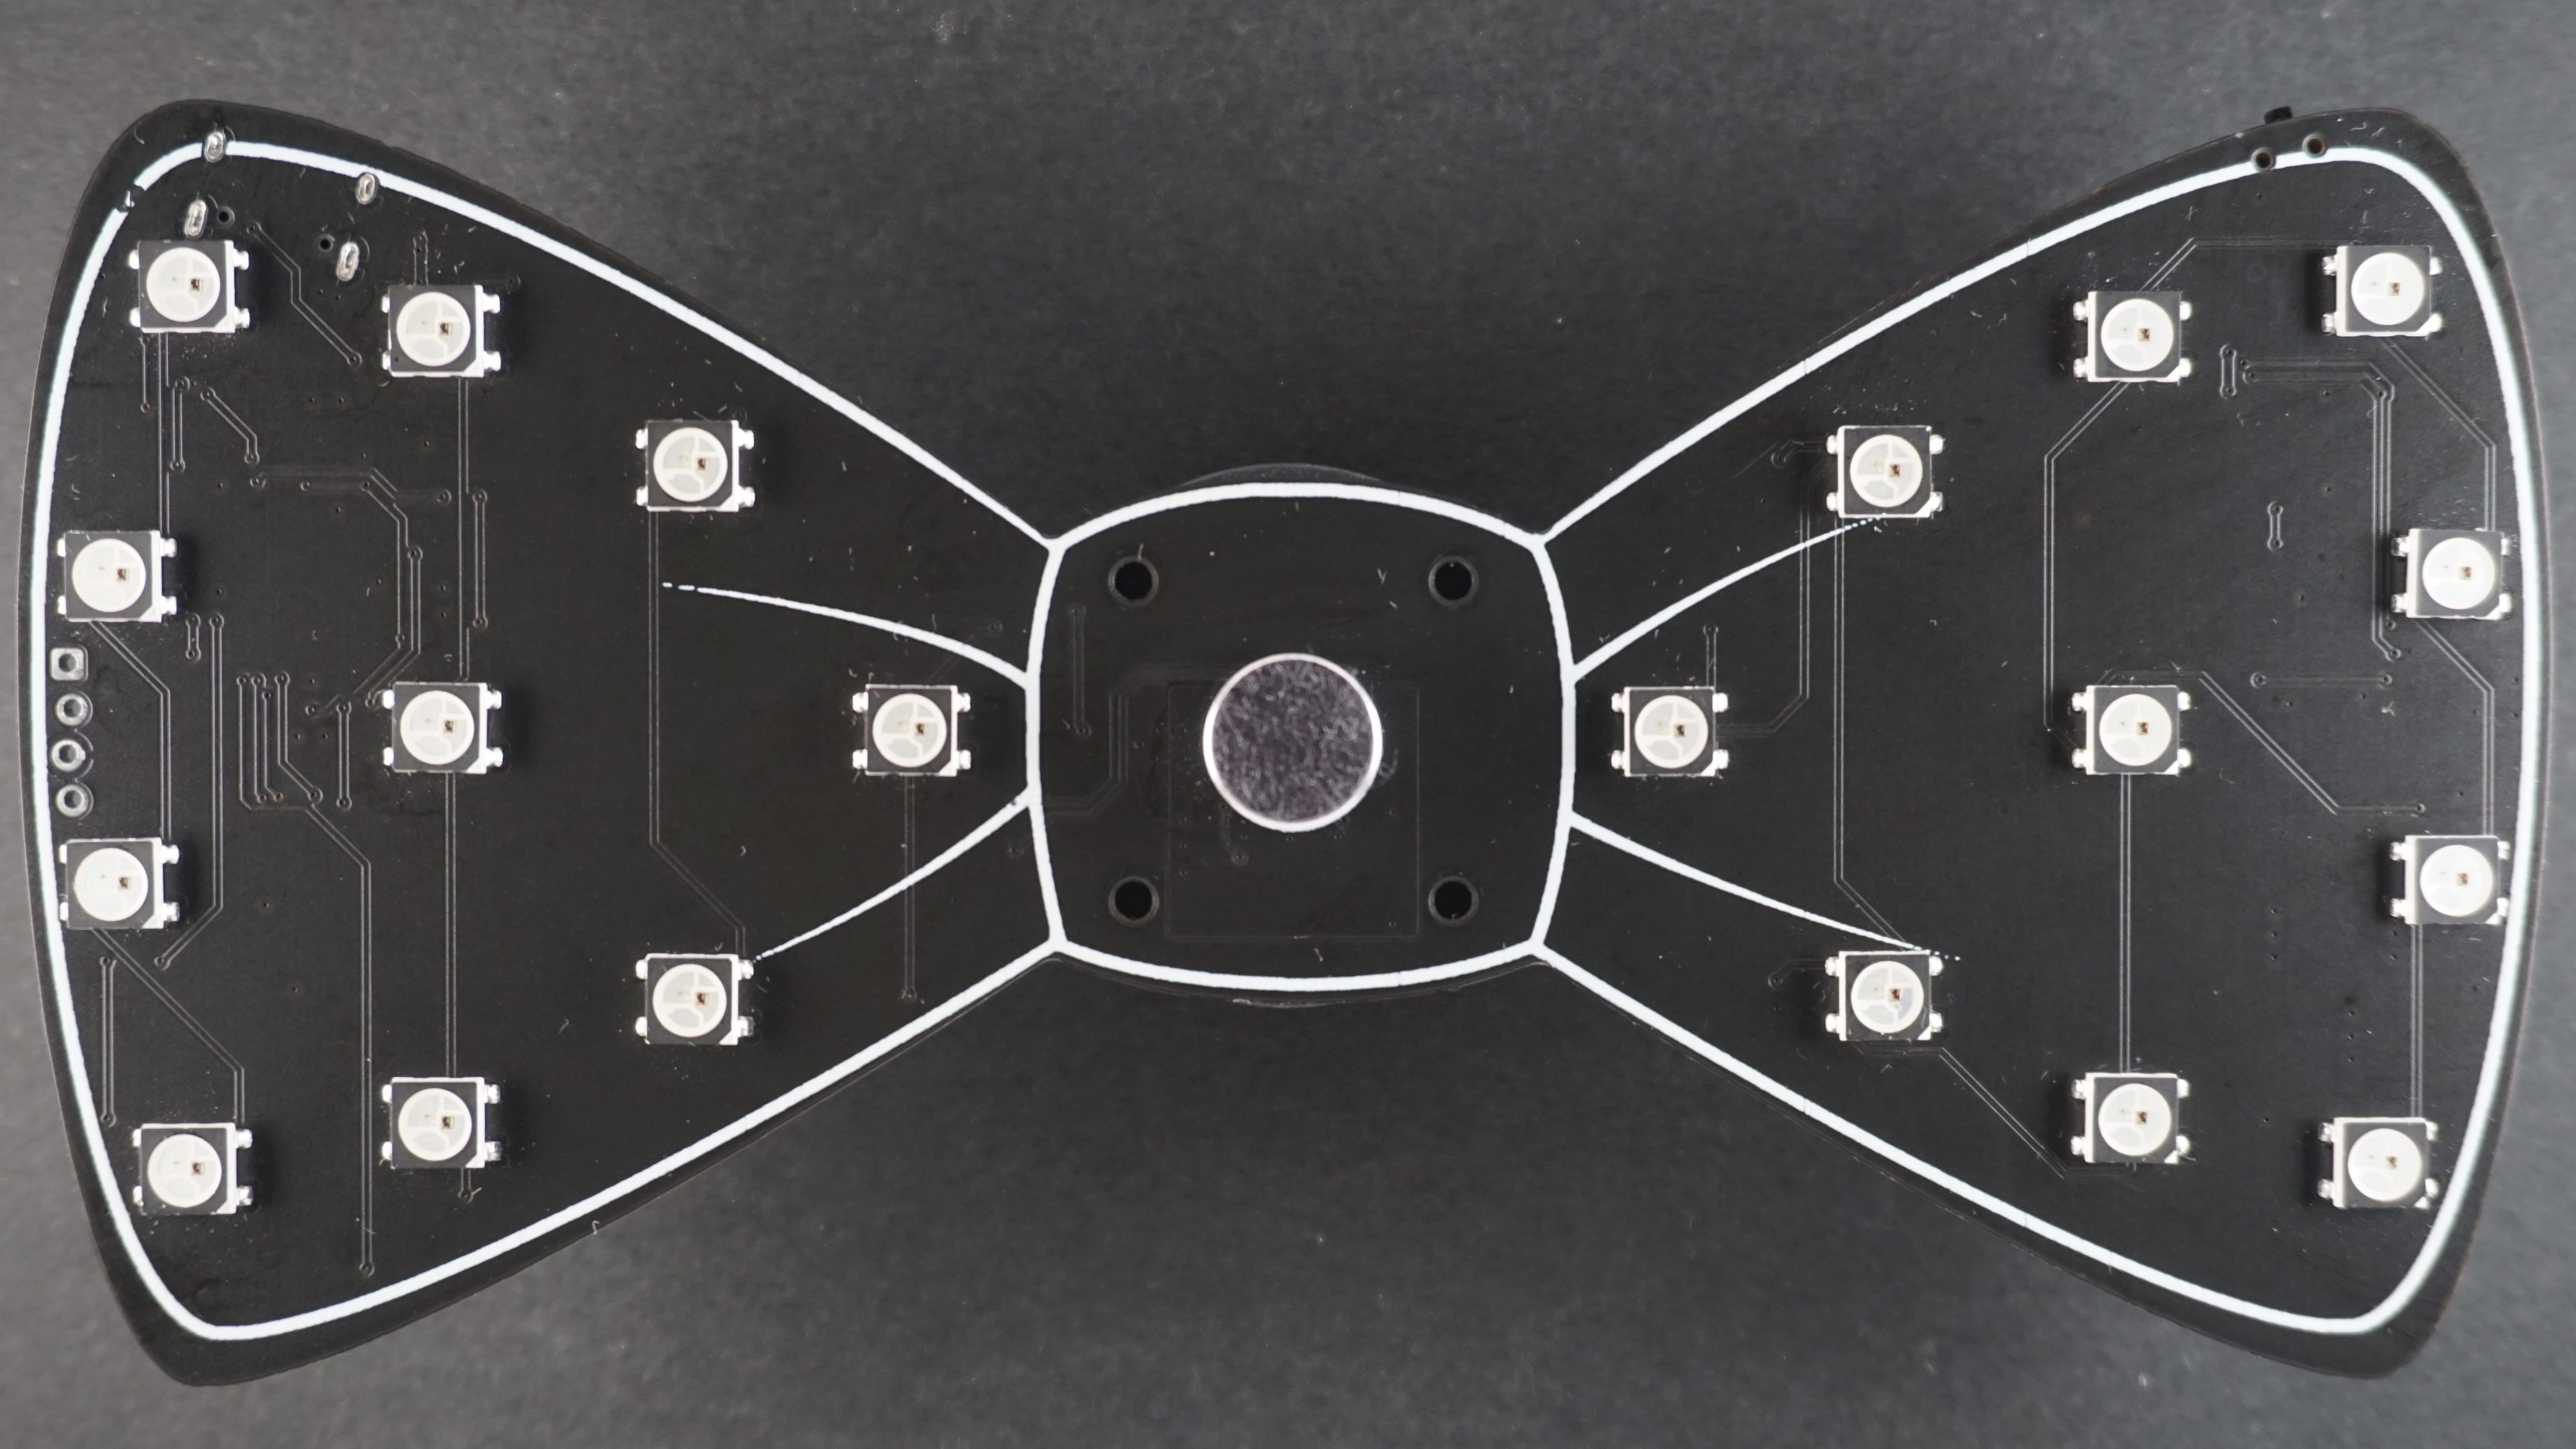
\includegraphics[width=0.9\linewidth]{images/bowtie-front.JPG}
			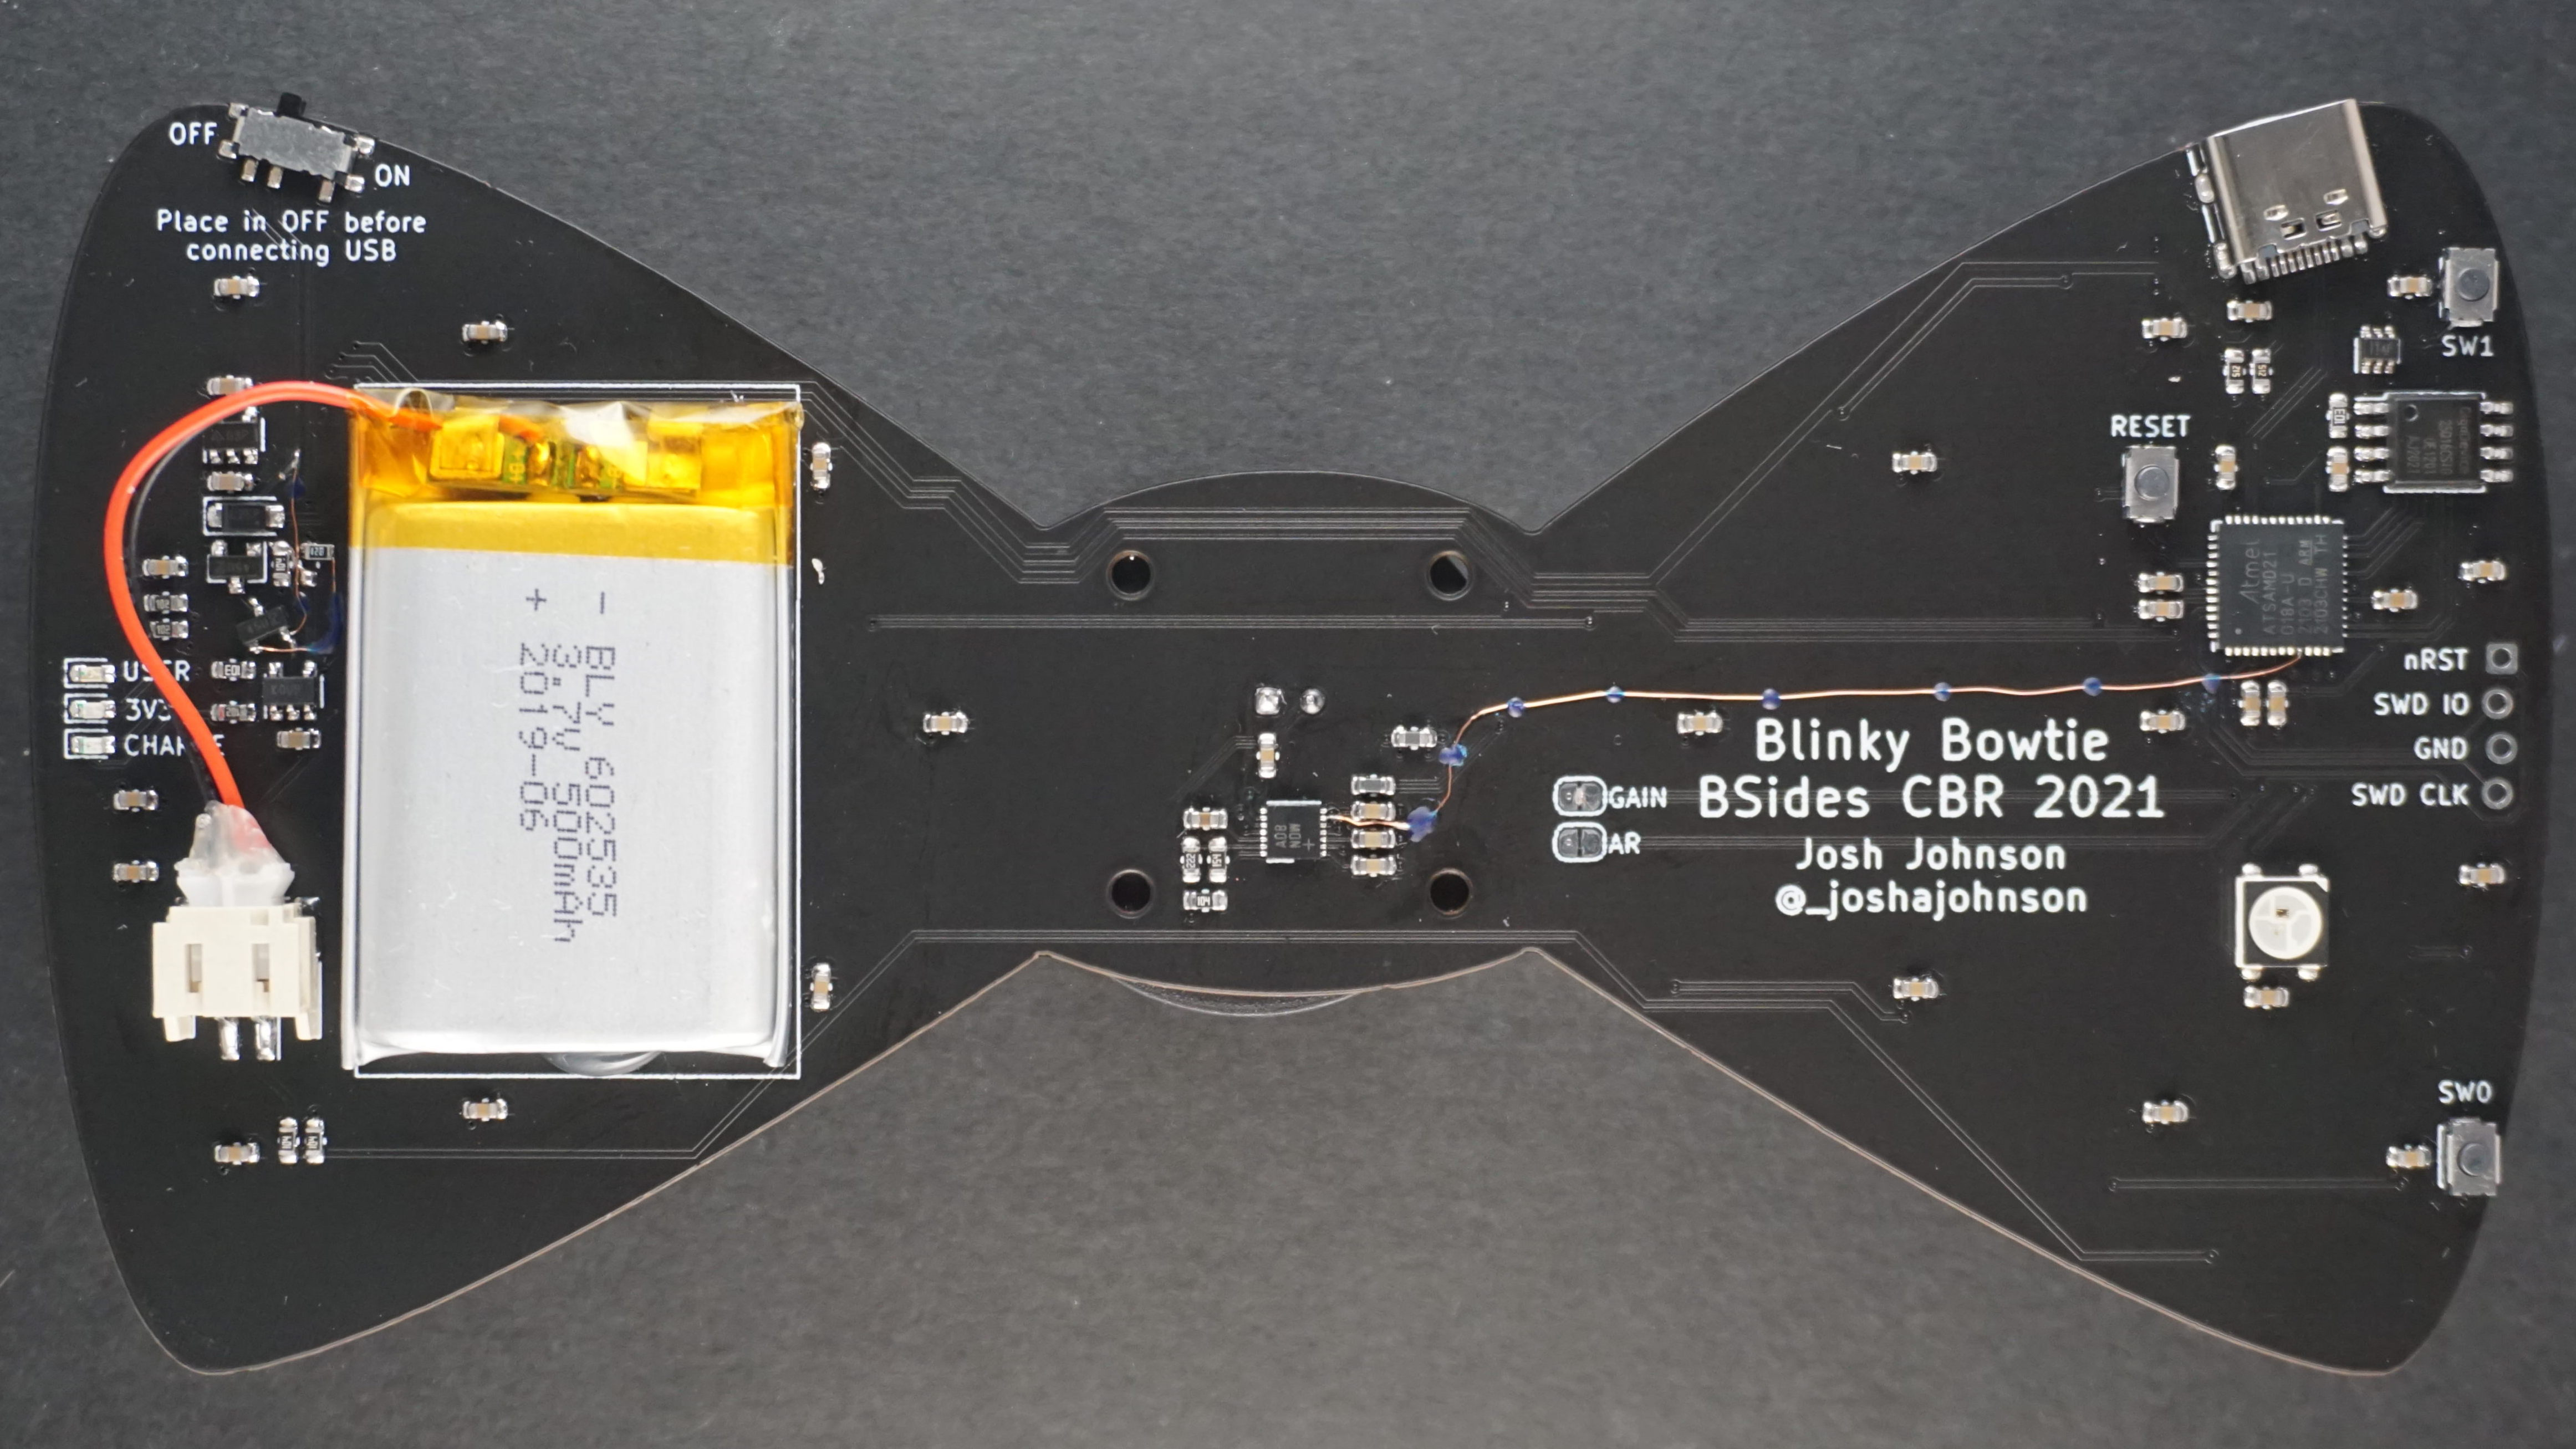
\includegraphics[width=0.9\linewidth]{images/bowtie-back.JPG}
		\end{figure}
\end{columns}
\end{frame}

%----------------------------------------------------------------------------------------
\begin{frame}
\frametitle{Requirements}
Depending on the objective of your design, there are a number of requirements / considerations which need to be taken into account as they will greatly impact your finished product. \\[10pt]

\begin{itemize}
	\item Physical dimensions / form factor
	\item Interacting with design (buttons, sensors, displays, LEDs)
	\item Connectivity (USB, Bluetooth, WiFi)
	\item Programming (bootloader, on board / external programmer, Arduino / C / Python)
	\item Power supply / battery
	\item Complexity (component size, COTS modules, part count)
	\item Assembly (through hole, surface mount, single vs double sided)
	\item Cost (PCB features, component selection)
\end{itemize}
\end{frame}

%----------------------------------------------------------------------------------------
\begin{frame}
\frametitle{Locating Resources / Reference Designs}
With requirements in hand, we can now start searching for suitable parts.\\
Evalulation boards are a great place to start, as they provide working hardware, documentation, and example code if applicable.\\[10pt]
\begin{columns}
	\column{.5\textwidth}
		\vspace{-7mm}
		\begin{itemize}
			\item Adafruit / Sparkfun
			\item Open Source Hardware (GitHub, Hackaday.io)
			\item Manufacturer Evaluation Boards
			\item Application Notes
			\item Datasheet
		\end{itemize}
		\vspace{2mm}
		All of the above will provide you with schematics and part numbers to kick start your design.

	\column{0.49\textwidth}
	\vspace{-8mm}
		\begin{figure}
			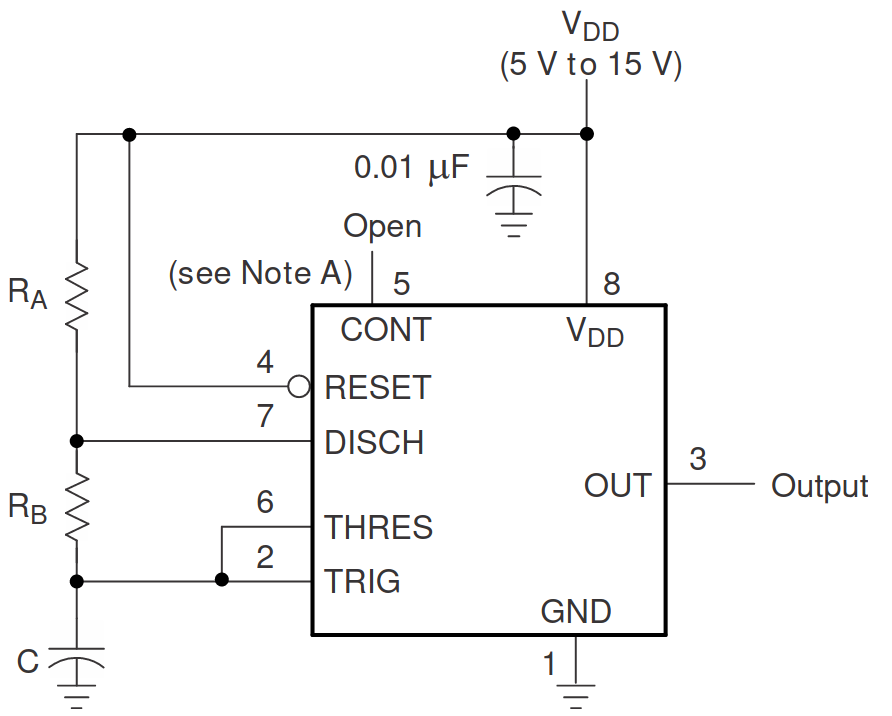
\includegraphics[width=0.8\linewidth]{images/tlc555-appnote.png}
		\end{figure}
\end{columns}
\end{frame}

%----------------------------------------------------------------------------------------
\begin{frame}
\frametitle{Schematic Capture}
\begin{columns}
	\column{.6\textwidth}
	What: Abstract representation of circuit / components.\\
	Why: Communicates purpose and documents design.\\
	How:
	\begin{itemize}
		\item Symbol creation
		\item Symbol placement
		\item Connect everything with wires
		\item Add notes to your design
		\item Run electrical rules checks (ERC)
		\item Footprint association (may be done in symbol placement)
		\item Bill of Materials (BOM) generation 
	\end{itemize}
	
	\column{0.39\textwidth}
	\vspace{-8mm}
	\begin{figure}
		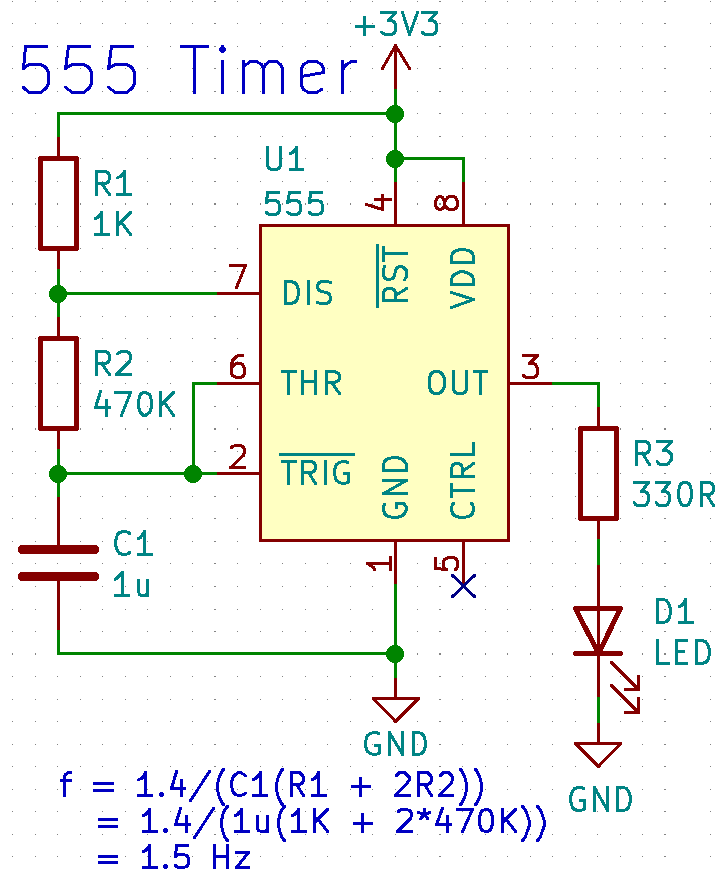
\includegraphics[width=\linewidth]{images/555-schematic-snip.png}
	\end{figure}
\end{columns}
\end{frame}

%----------------------------------------------------------------------------------------
\begin{frame}
	\frametitle{Parts of a PCB}
	\vspace{-2mm}
	\begin{figure}
		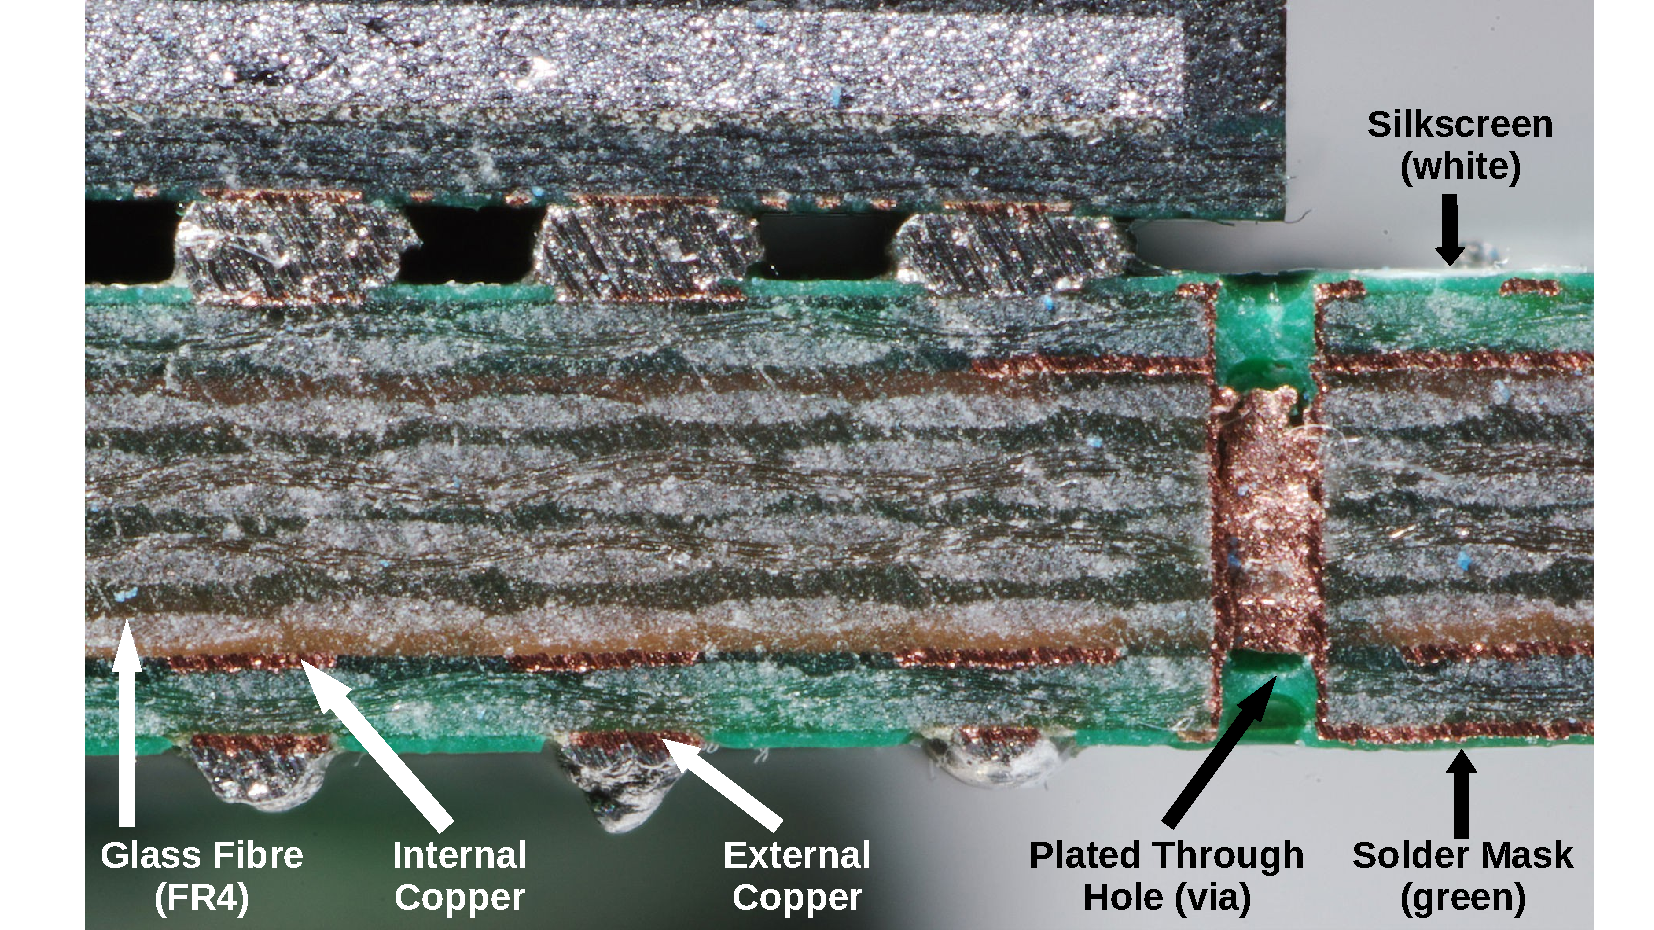
\includegraphics[width=12cm]{images/pcb-cross-section-markup.pdf}
		\text{Image: Rainer Knäpper}
	\end{figure}
\end{frame}

%----------------------------------------------------------------------------------------
\begin{frame}
\frametitle{PCB Layout}
\begin{columns}
	\column{.6\textwidth}
	What: Physical representation of circuit / components.\\
	Why: Ensures electrical and mechanical function.\\
	How:
	\begin{itemize}
		\item Configure design rules per manufacturer guidelines
		\item Draw board outline
		\item Place connectors and mounting holes
		\item Place electronic components
		\item Route critical nets, power, then everything else
		\item Run design rule checks (DRC)
		\item Add decorative features
		\item Review in 3D viewer / check mechanical fit
		\item Export Gerbers
	\end{itemize}
	
	\column{0.39\textwidth}
	\vspace{-7mm}
	\begin{figure}
		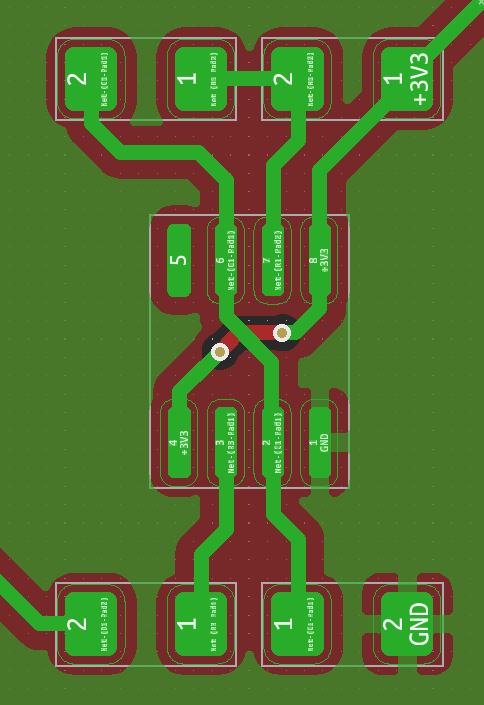
\includegraphics[width=0.8\linewidth]{images/555-layout.png}
	\end{figure}
\end{columns}
\end{frame}

%----------------------------------------------------------------------------------------
\begin{frame}
\frametitle{Ordering PCBs / Components}
\begin{columns}
	\column{.5\textwidth}
	PCB
	\begin{itemize}
		\item Check Gerbers were exported correctly
		\item Zip up Gerbers
		\item Upload to manufacturer
		\item Choose PCB options (quantity, colour, surface finish)
	\end{itemize}
	
	\column{0.49\textwidth}
	Components
	\begin{itemize}
		\item Export BOM from Schematic
		\item Upload to supplier
		\item Confirm package size is correct
		\item Confirm availability before ordering boards!
	\end{itemize}
	
\end{columns}
\vspace{5mm}
\begin{figure}
	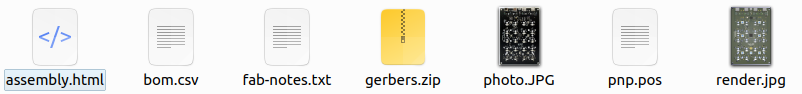
\includegraphics[width=\linewidth]{images/exported-files.png}
\end{figure}
\end{frame}

%----------------------------------------------------------------------------------------
\begin{frame}
\frametitle{Assembly}
You have all the parts, but how to put them together?
\begin{itemize}
	\item Development Boards - point to point or wired through a breadboard
	\item Through Hole - solder with a soldering iron
	\item Surface Mount - reflow with a stencil and solder paste, or solder with an iron
	\item All - ask your PCB manufacturer to do it for you (even in small volumes)
\end{itemize}
\vspace{-5mm}
\begin{columns}
	\column{.5\textwidth}
	\begin{figure}
		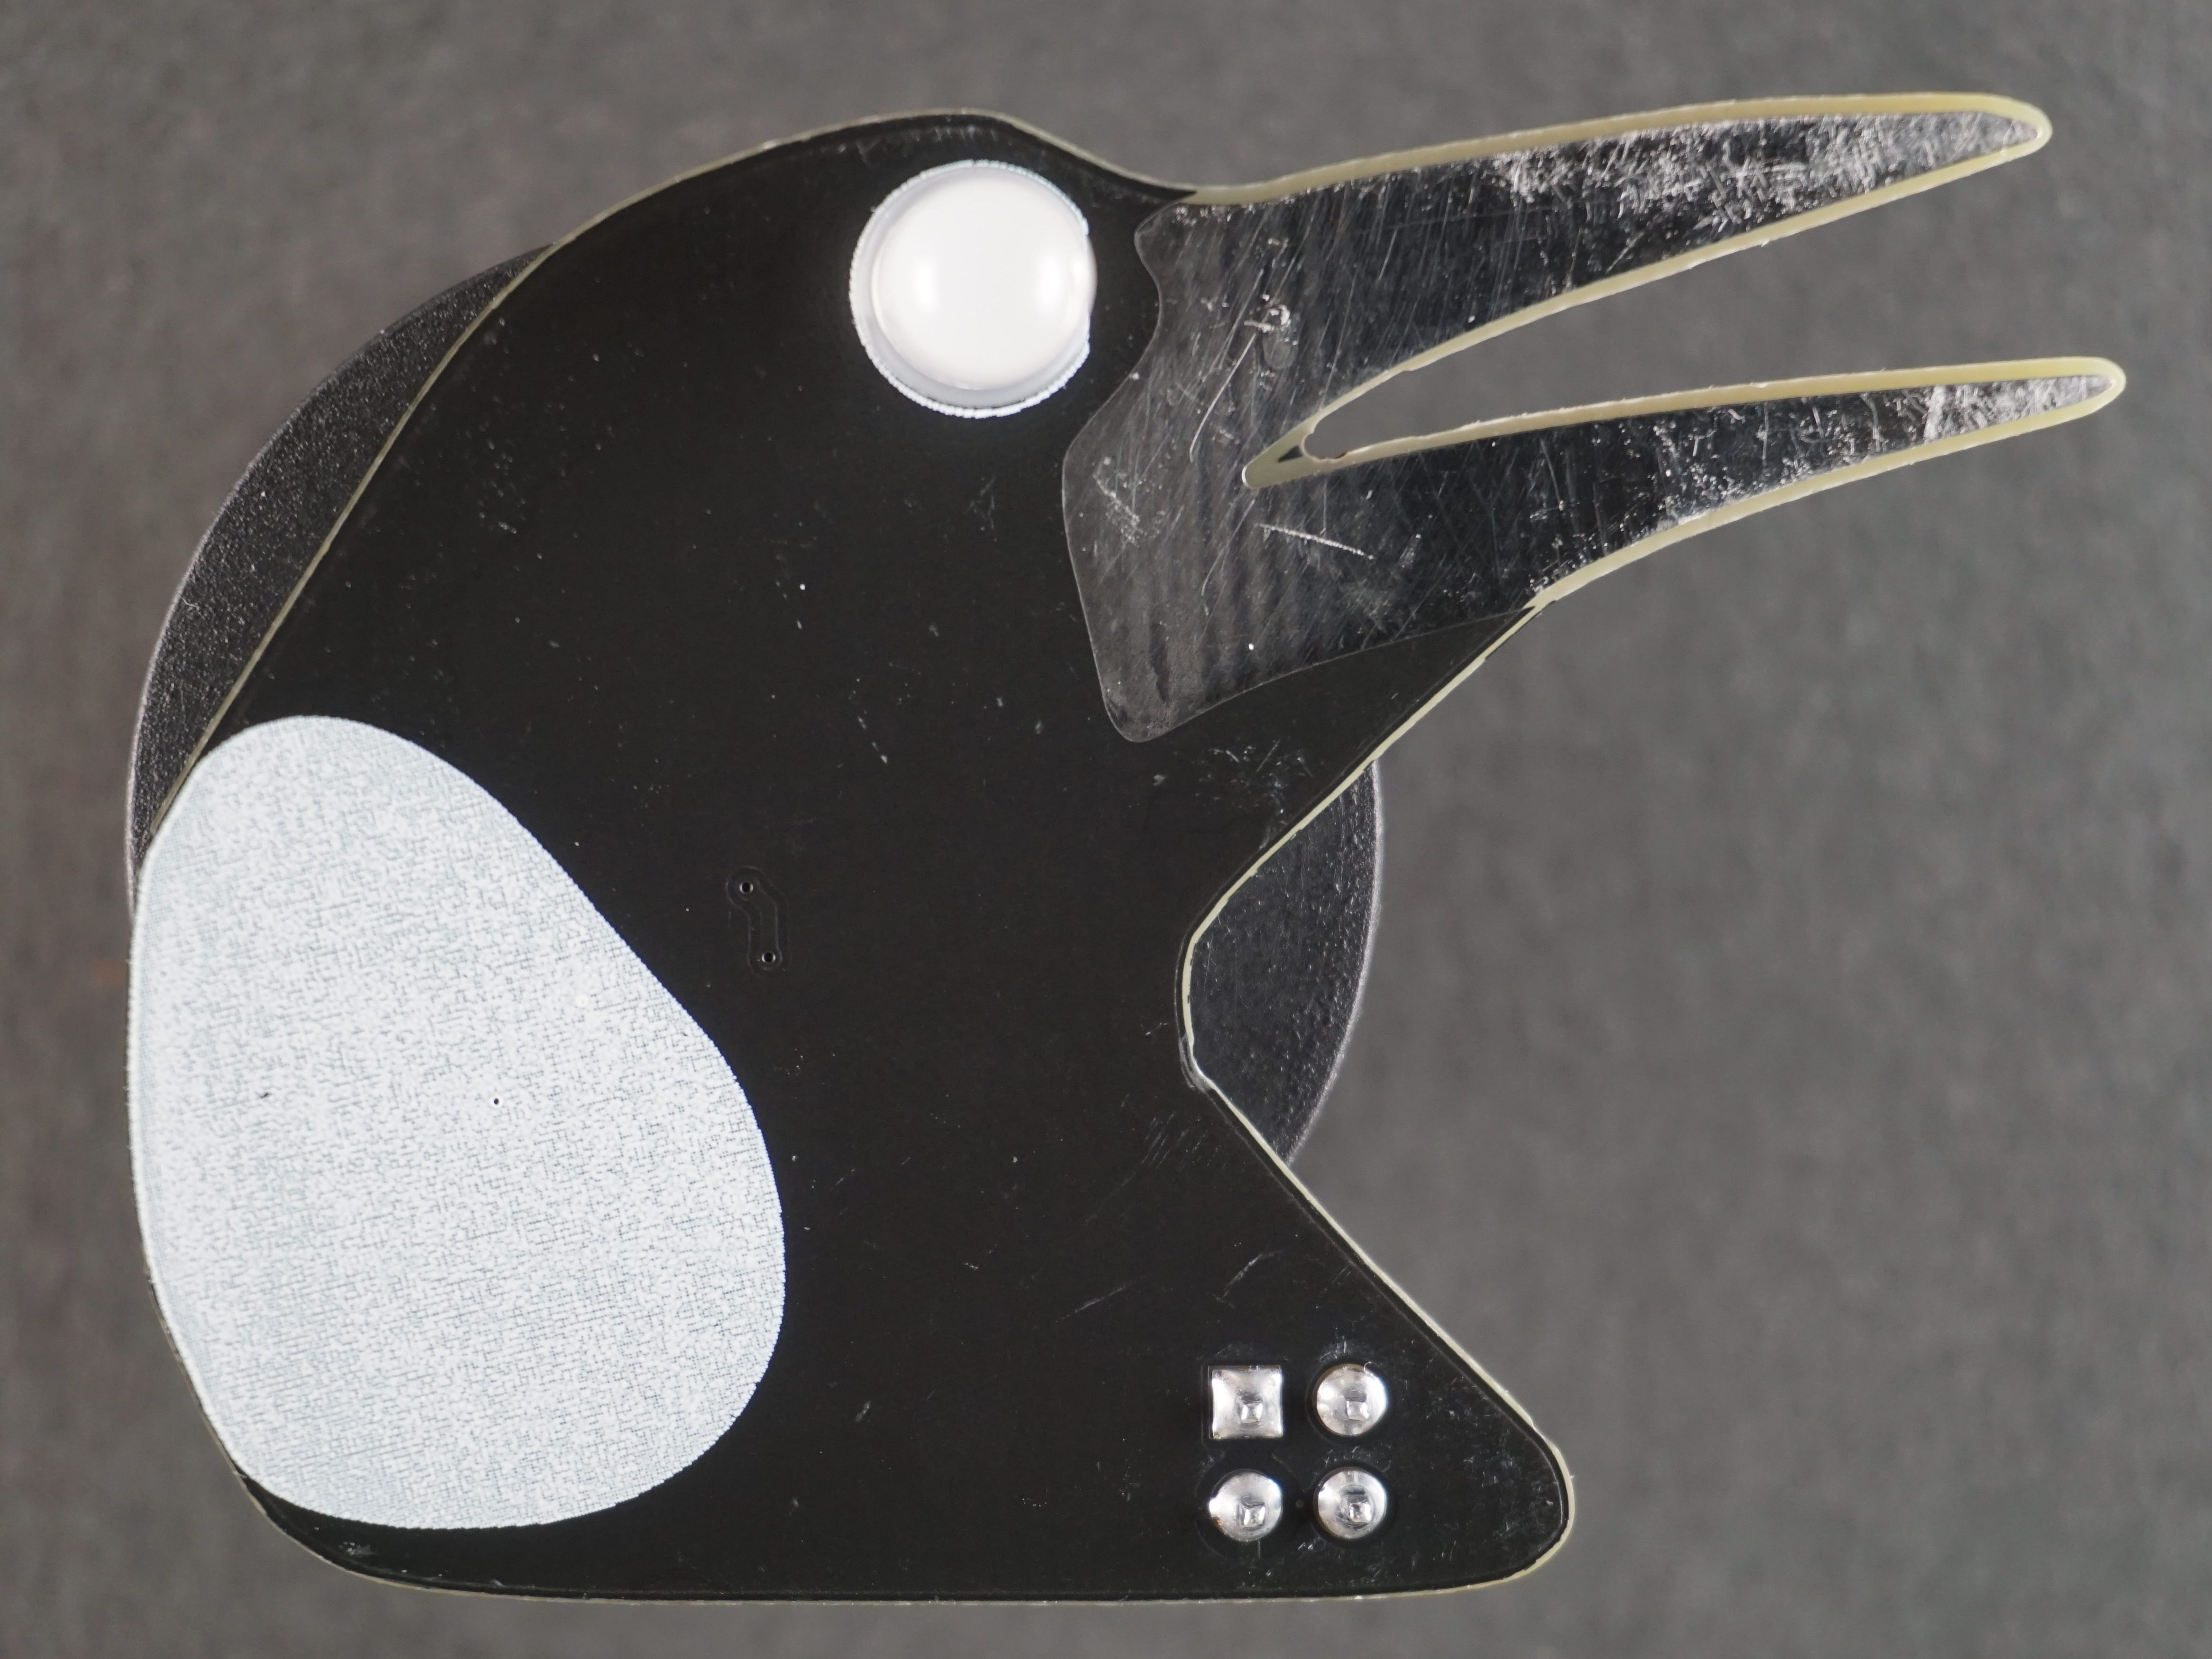
\includegraphics[height=4cm]{images/magpie-front.JPG}
	\end{figure}
	\column{0.49\textwidth}
	\begin{figure}
		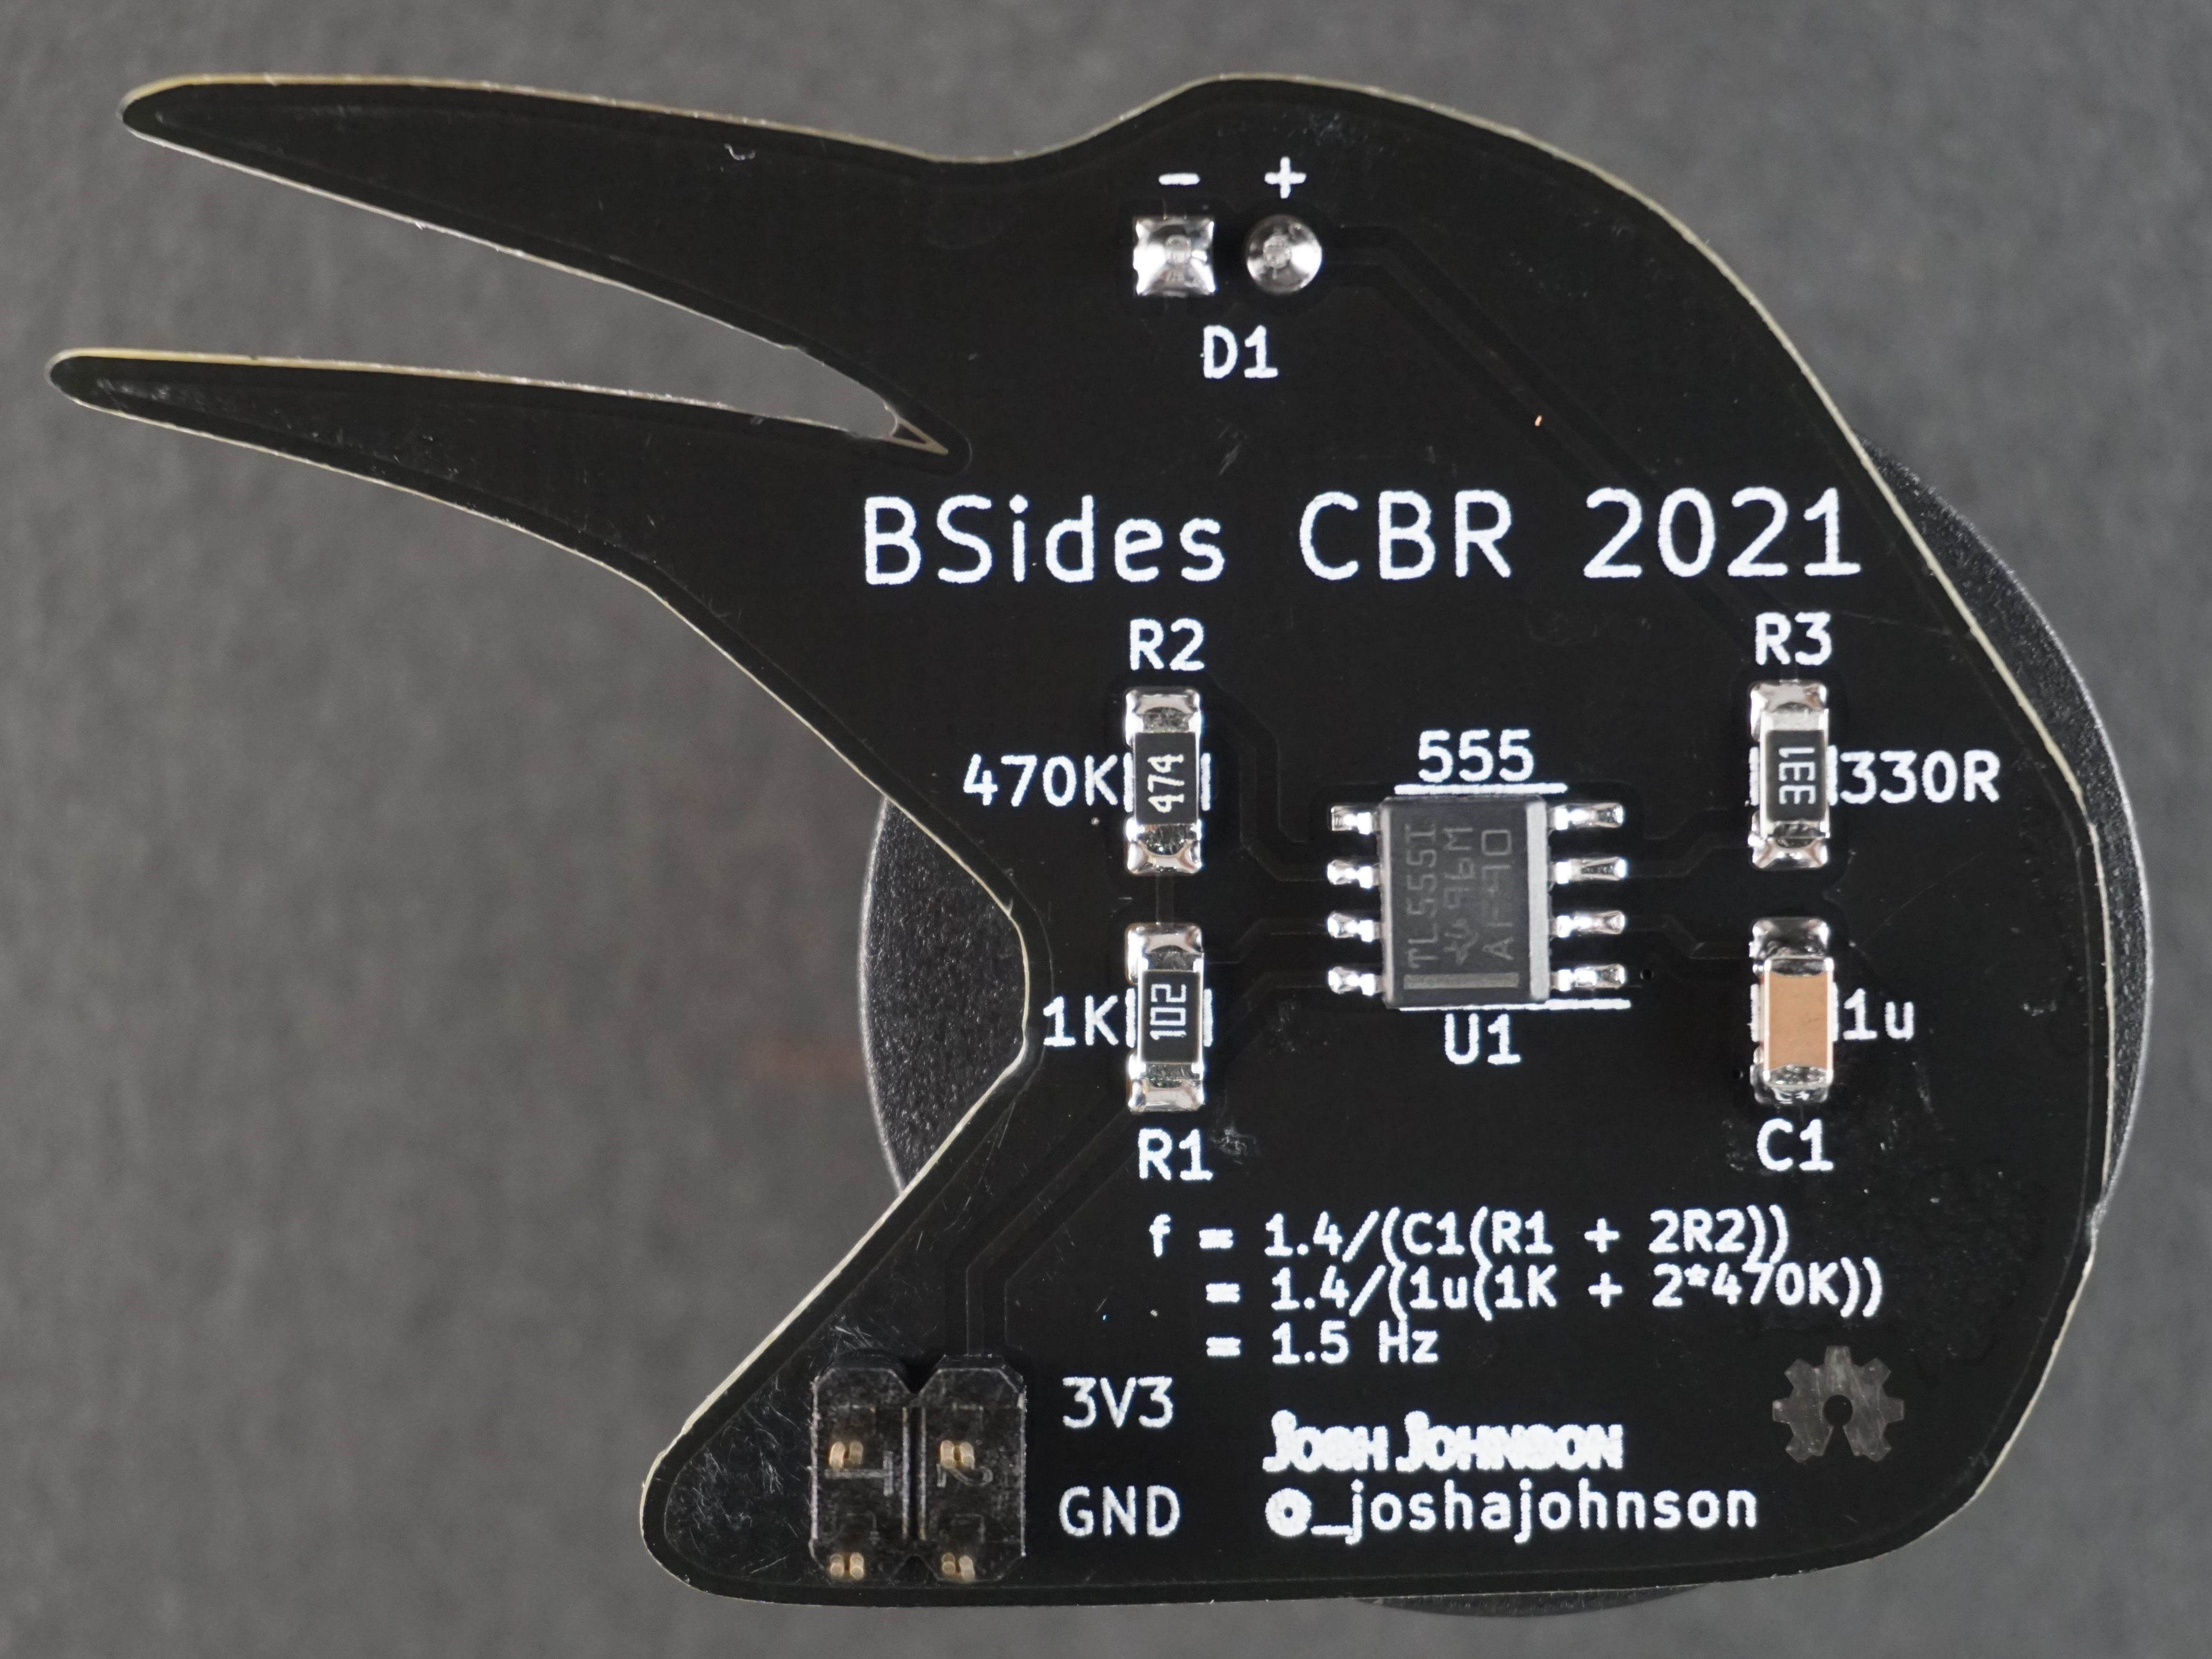
\includegraphics[height=4cm]{images/magpie-back.JPG}
	\end{figure}
\end{columns}
\end{frame}

%----------------------------------------------------------------------------------------
\begin{frame}
\frametitle{Example - Sound Reactive LEDs - Breadboard Prototype}
\vspace{-5mm}
\begin{columns}
	\column{.5\textwidth}
	\begin{itemize}
		\item Ideal for: Confirming compenents will work as required for your project, or one off builds.
		\item Wired components following a guide from Adafruit.
		\item Adafruit M0 Feather, Microphone, WS2812 (Neopixel) strip, MPU6050 IMU.
		\item If things don't work (like the IMU), easy to remove.
		\item Pros: Great for prototyping.
		\item Cons: Challenging to meet mechanical requirements, fiddly to assemble.
	\end{itemize}
	\column{0.49\textwidth}
	\begin{figure}
		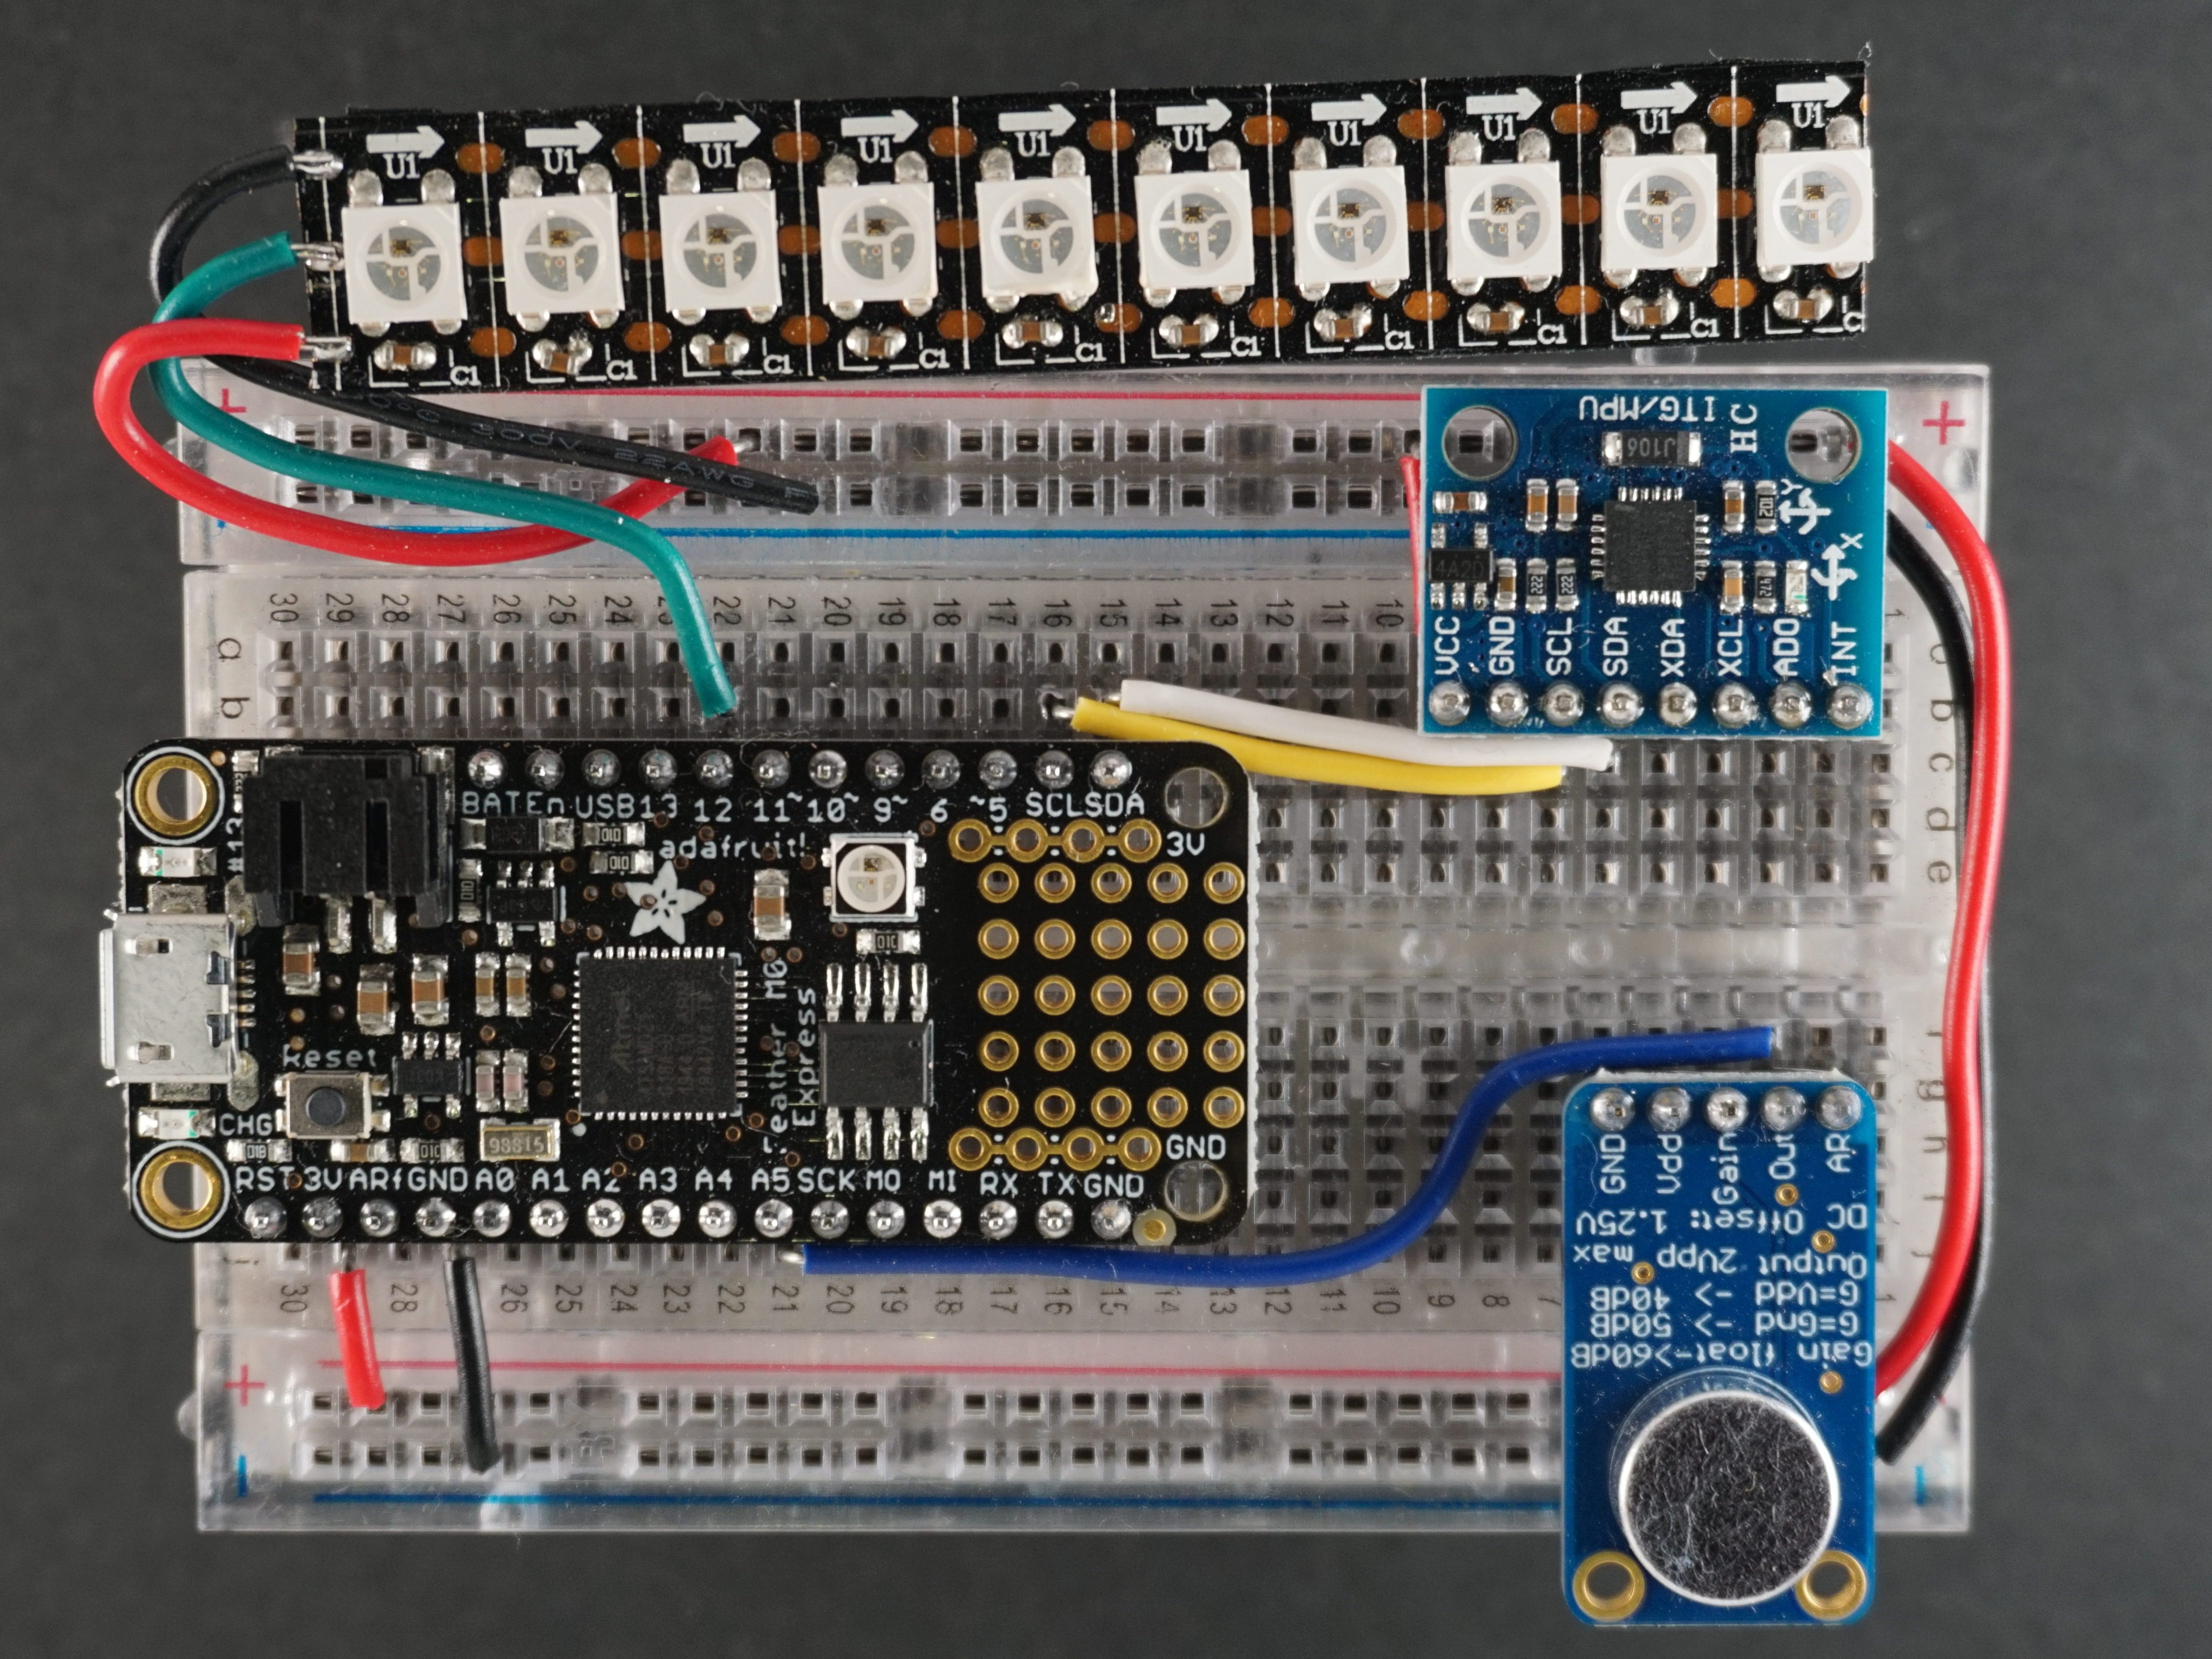
\includegraphics[width=\linewidth]{images/breadboard.JPG}
	\end{figure}
\end{columns}
\end{frame}

%----------------------------------------------------------------------------------------
\begin{frame}
\frametitle{Example - Sound Reactive LEDs - Through Hole PCB}
\vspace{-5mm}
\begin{columns}
	\column{.5\textwidth}
	\begin{itemize}
		\item Ideal for: Non space constrained / low volume designs / prototyping.
		\item Replaced wires on breadboard with traces on PCB.
		\item Identical wiring and firmware to breadboard prototype.
		\item Four unique parts, low risk of PCB design errors.
		\item Pros: Quick and easy to assemble and bring up, low part count, low complexity.
		\item Cons: Expensive to manufacture in volume, challenging to make small.
	\end{itemize}
	\column{0.49\textwidth}
	\begin{figure}
		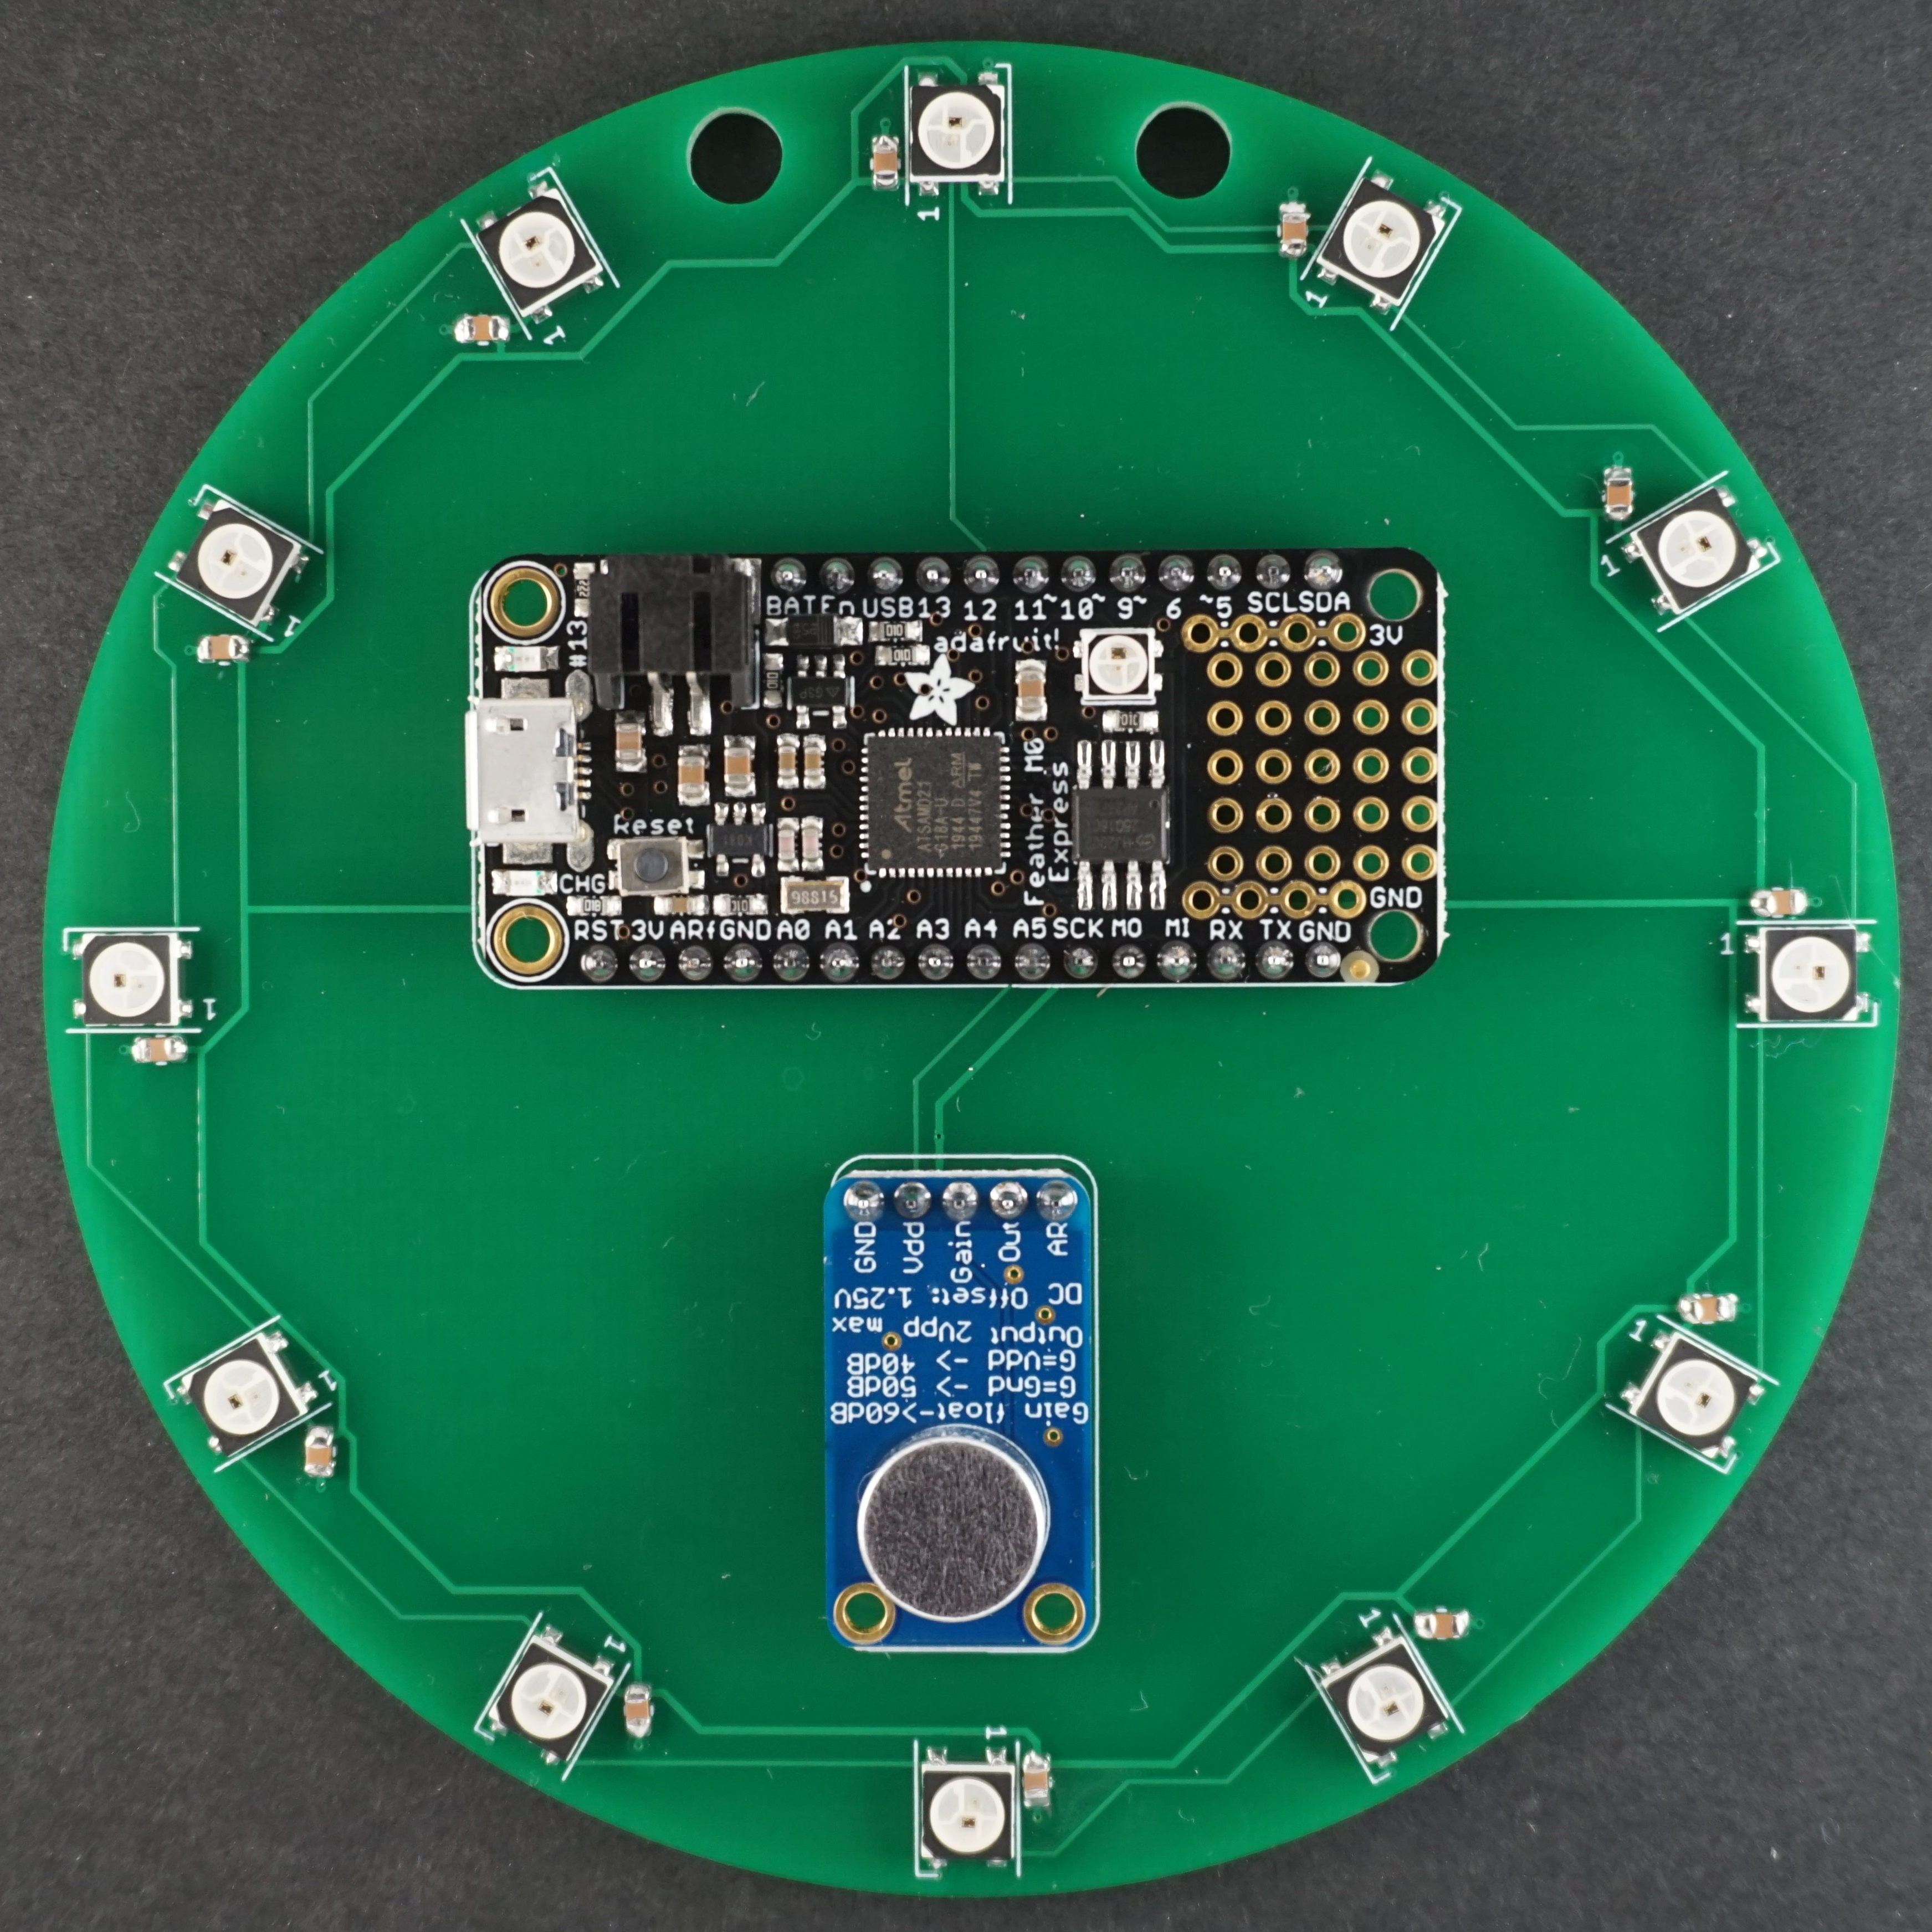
\includegraphics[width=0.9\linewidth]{images/circle-feather.JPG}
	\end{figure}
\end{columns}
\end{frame}

%----------------------------------------------------------------------------------------
\begin{frame}
\frametitle{Through Hole PCB - Schematic}
\vspace{-5mm}
\begin{columns}
	\column{.4\textwidth}
	\begin{itemize}
		\item Replicating breadboard wiring in schematic.
		\item All but microphone in KiCad Library, can use a simple 1x5 connector.
		\item Added a PCB jumper to change gain if required.
		\item Known good circuit, so low risk of issues.
		\item Four unique parts, 26 parts total.
	\end{itemize}
	\column{0.59\textwidth}
	\begin{figure}
		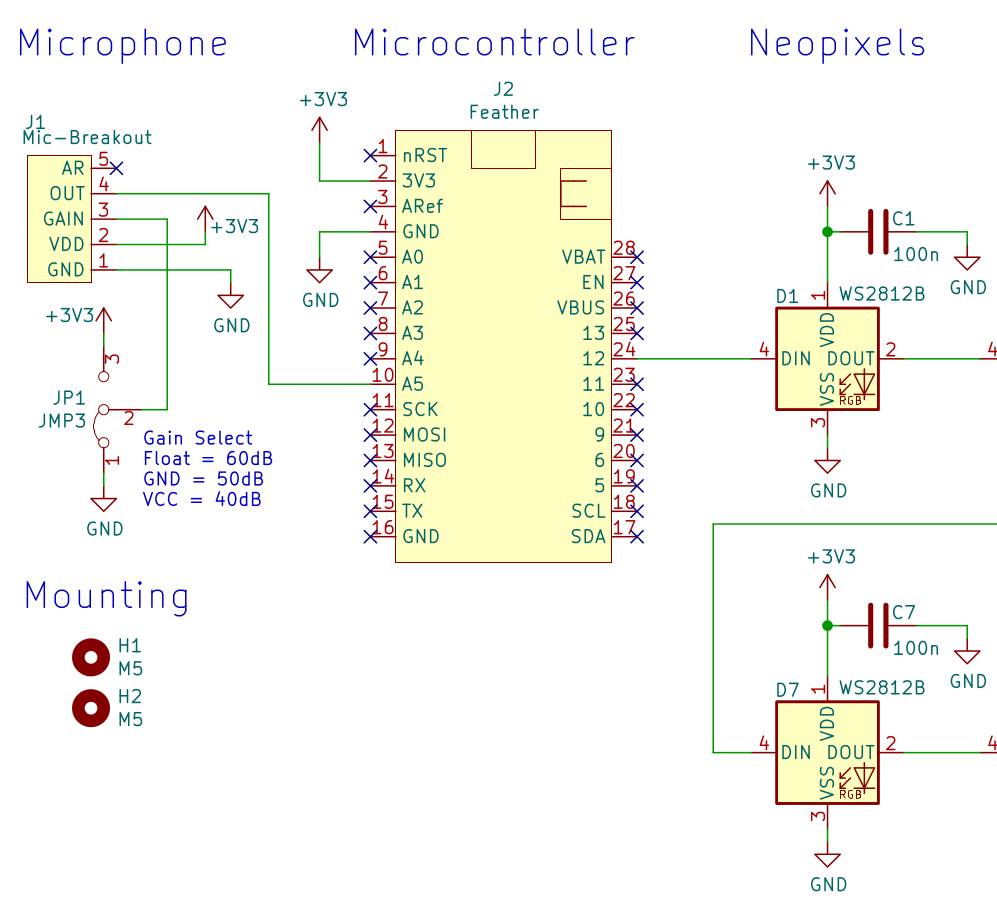
\includegraphics[width=0.9\linewidth]{images/module-schematic.png}
	\end{figure}
\end{columns}
\end{frame}

%----------------------------------------------------------------------------------------
\begin{frame}
\frametitle{Through Hole PCB - Layout}
\vspace{-5mm}
\begin{columns}
	\column{.5\textwidth}
	\begin{itemize}
		\item Two layer board, ground pour on bottom, signals and power on top.
		\item Through hole or large surface mount devices (SMD).
		\item Simple board outline drawn using the circle tool.
		\item Mounting points added to attach lanyard to.
	\end{itemize}
	\column{0.49\textwidth}
	\begin{figure}
		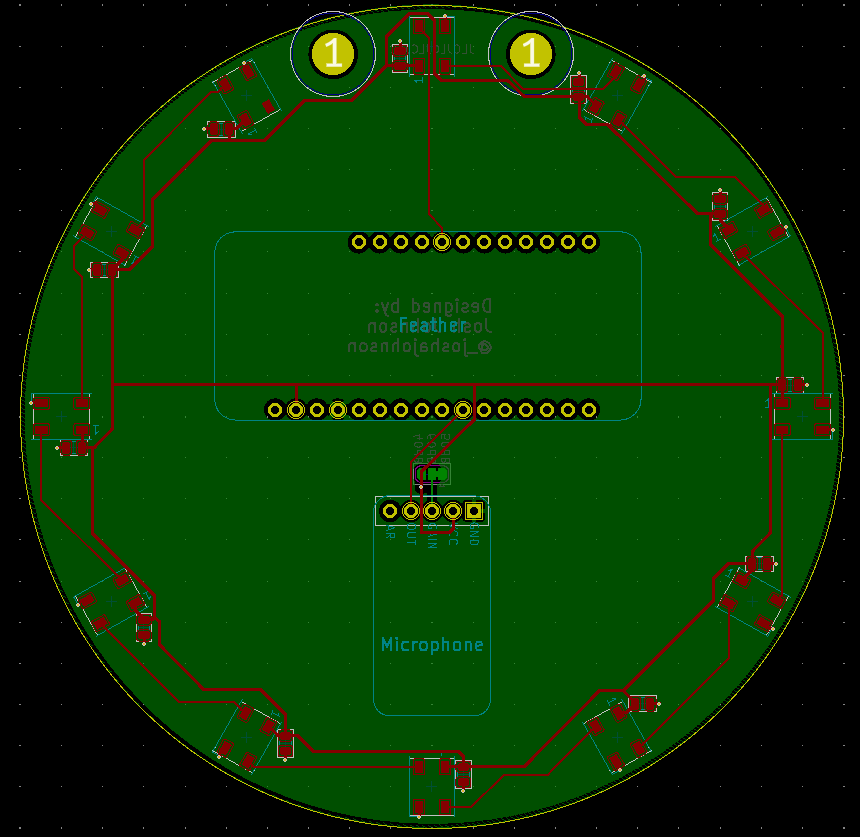
\includegraphics[width=0.9\linewidth]{images/module-layout.png}
	\end{figure}
\end{columns}
\end{frame}

%----------------------------------------------------------------------------------------
\begin{frame}
\frametitle{Through Hole PCB - Assembly}
\vspace{-5mm}
\begin{columns}
	\column{.5\textwidth}
	\begin{itemize}
		\item Hand assembled in an hour.
		\item Soldering iron only, no hot air gun.
		\item Firmware was loaded over USB just like breadboard.
		\item One mistake was made - microphone outline is 180$^\circ$ out and fixed after this photo.
	\end{itemize}
	\column{0.49\textwidth}
	\begin{figure}
		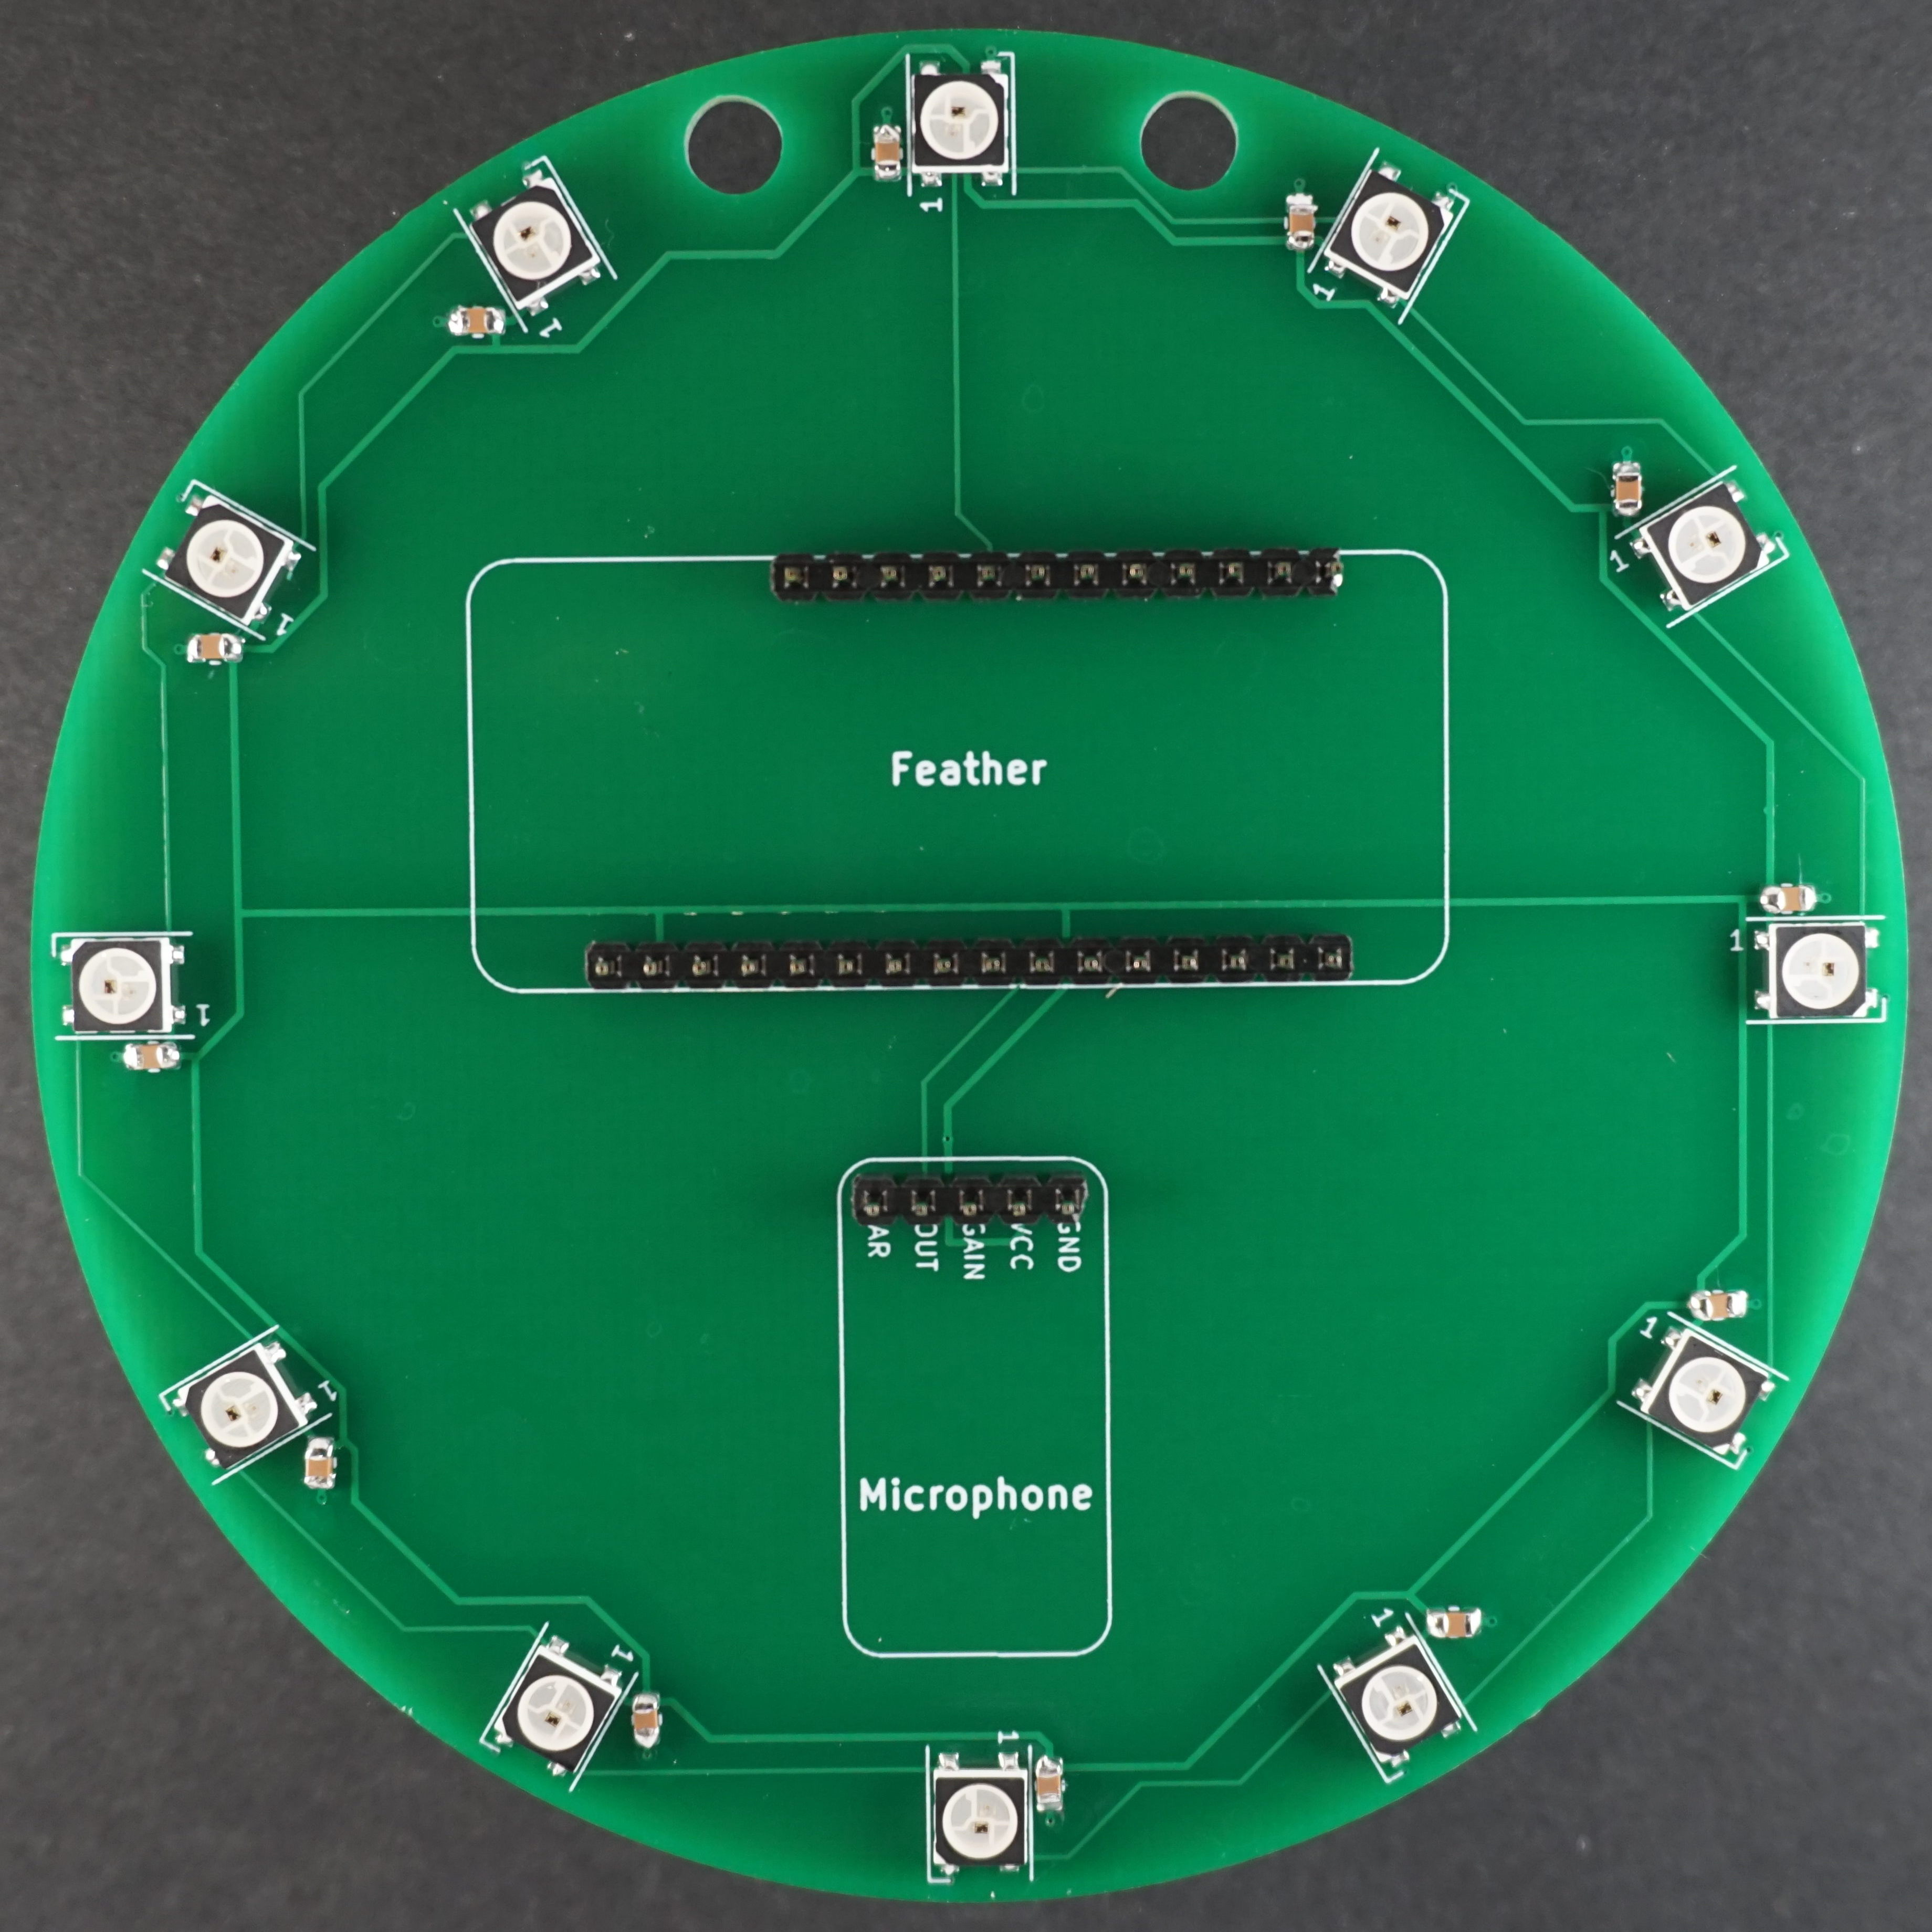
\includegraphics[width=0.9\linewidth]{images/circle-bare.JPG}
	\end{figure}
\end{columns}
\end{frame}

%----------------------------------------------------------------------------------------
\begin{frame}
\frametitle{Example - Sound Reactive LEDs - Integrated Design}
\vspace{-5mm}
\begin{columns}
	\column{.5\textwidth}
	\begin{itemize}
		\item Ideal for: Mechanically constrained / high volume designs.
		\item Ground up schematic capture and layout.
		\item If designed correctly, compatiable with prototype firmware.
		\item Higher risk of design errors, especially if designed after midnight...
		\item Pros: Guaranteed to suit mechanical requirements, easier / cheaper to produce in volume.
		\item Cons: More time required to design, assemble and bring up prototypes, harder to troubleshoot issues.
	\end{itemize}
	\column{0.49\textwidth}
	\begin{figure}
		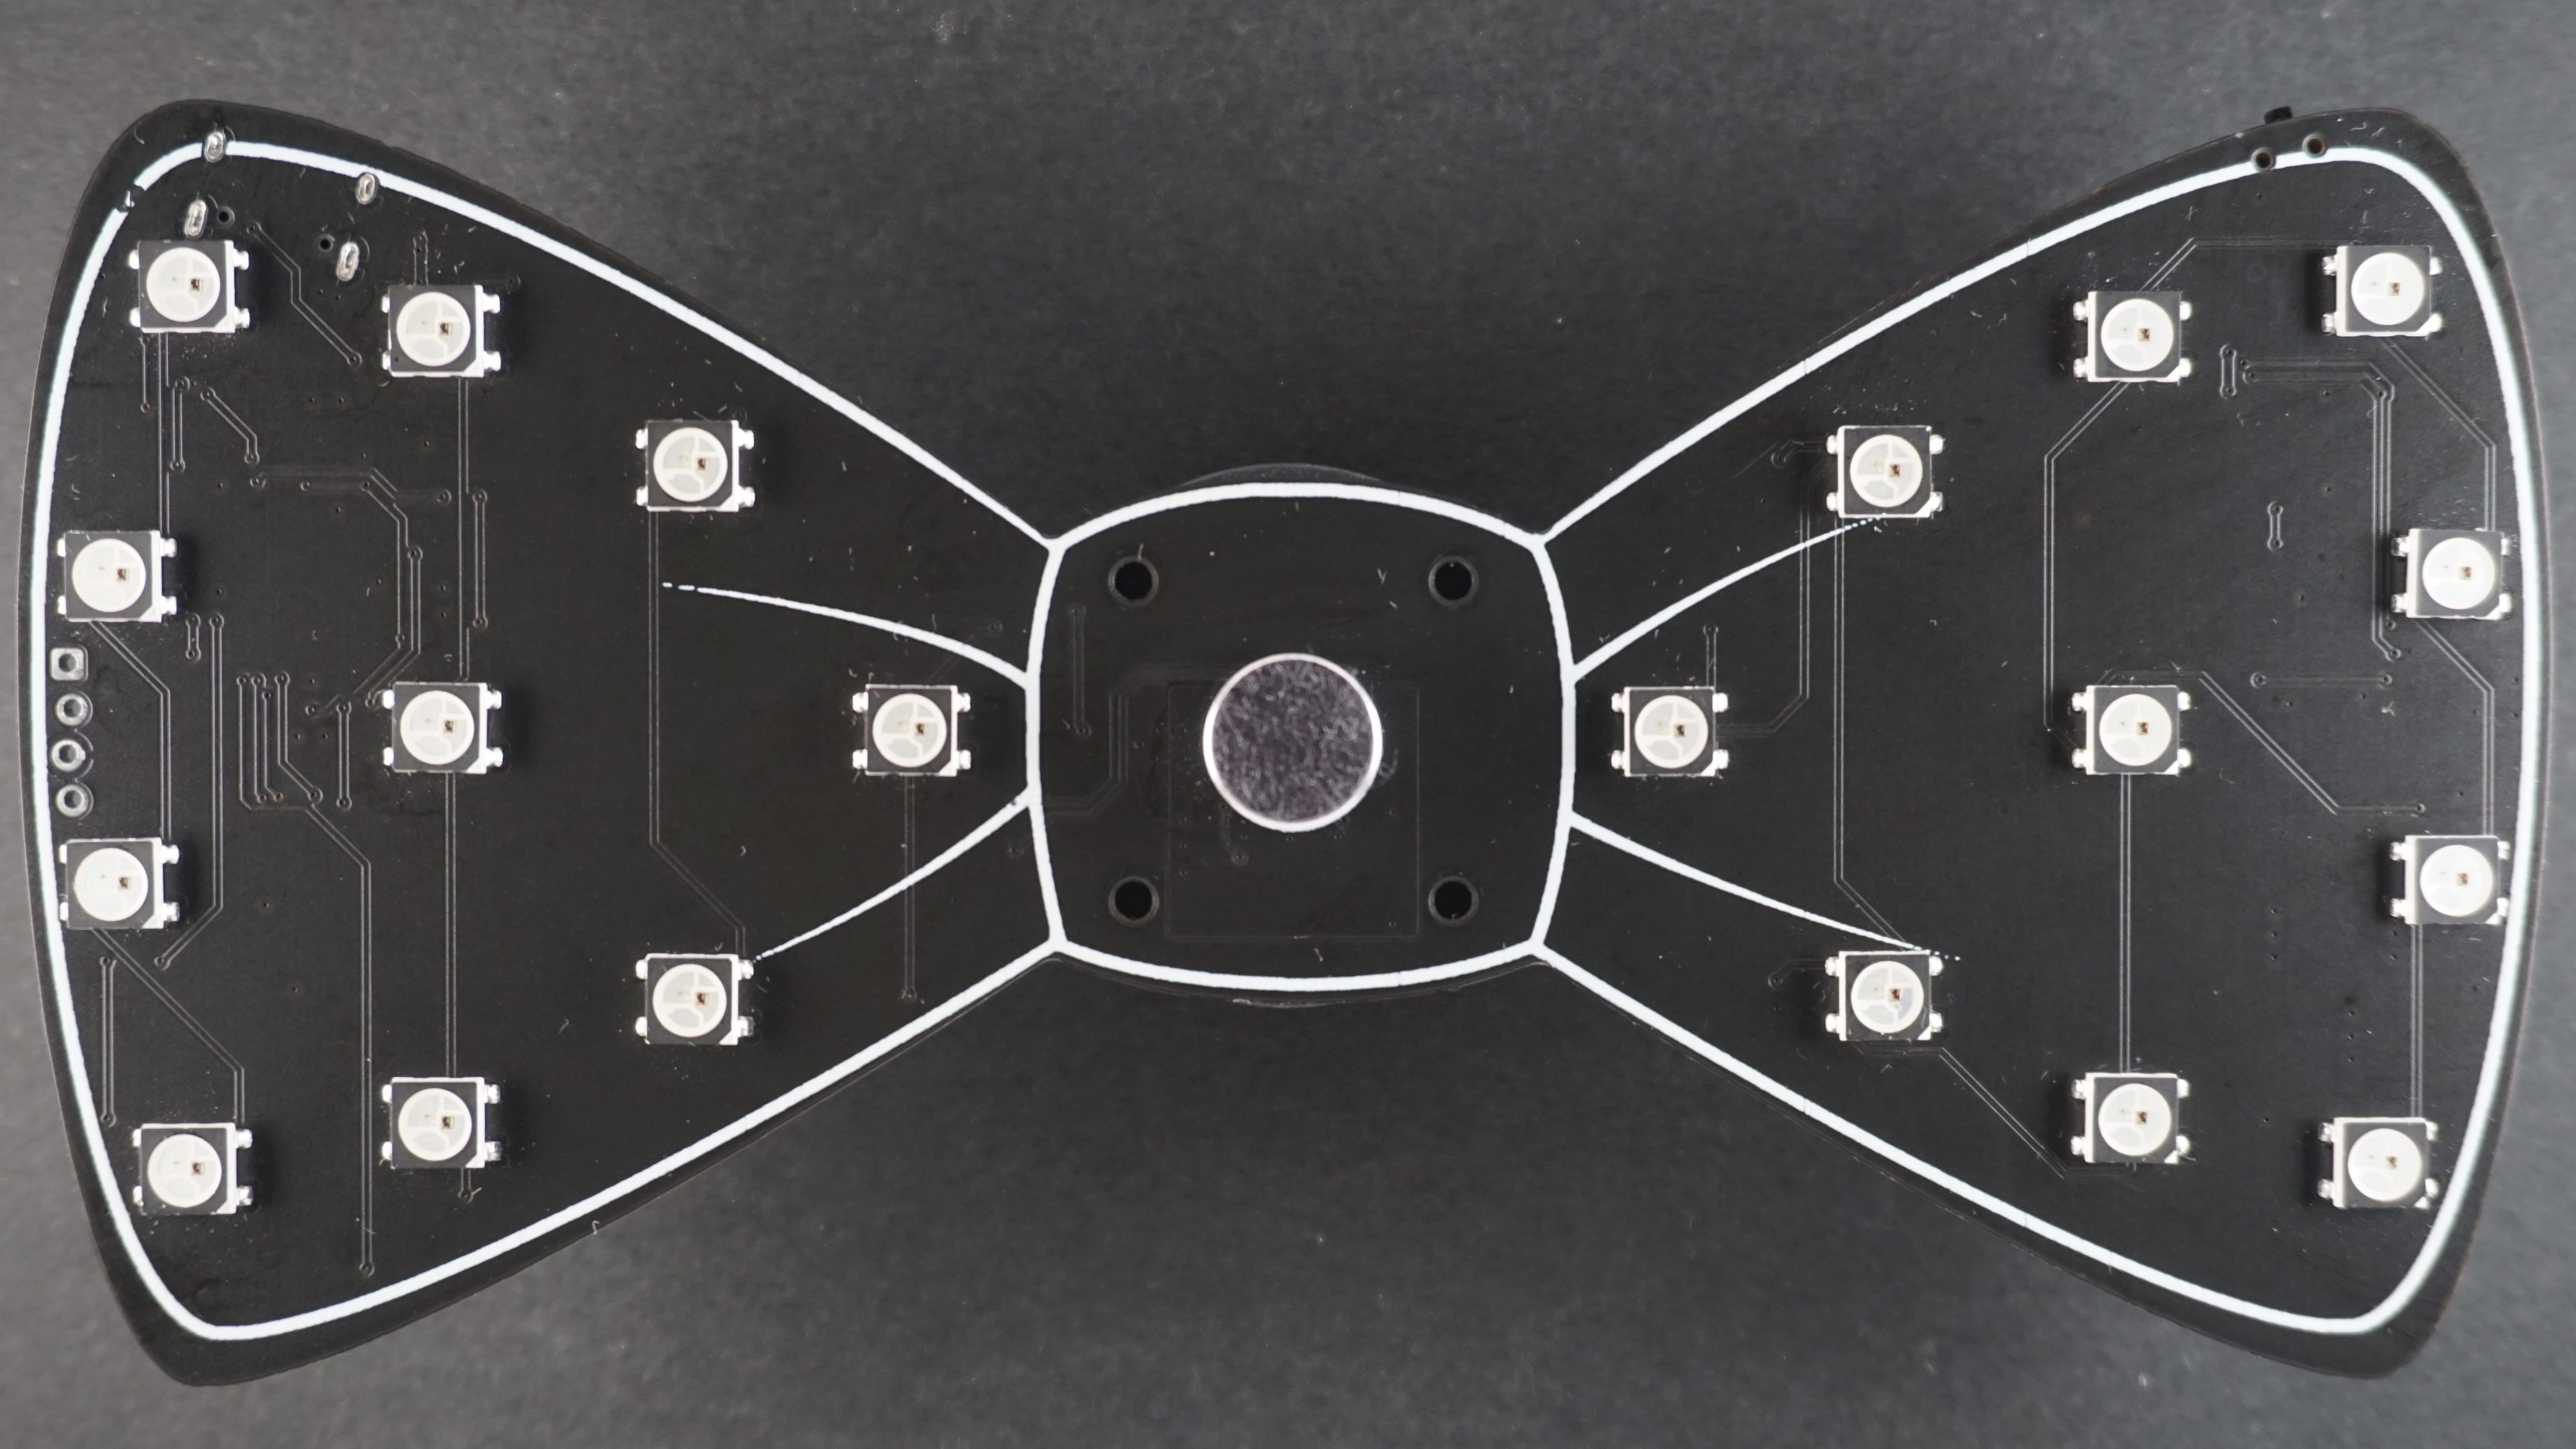
\includegraphics[width=0.8\linewidth]{images/bowtie-front.JPG}
		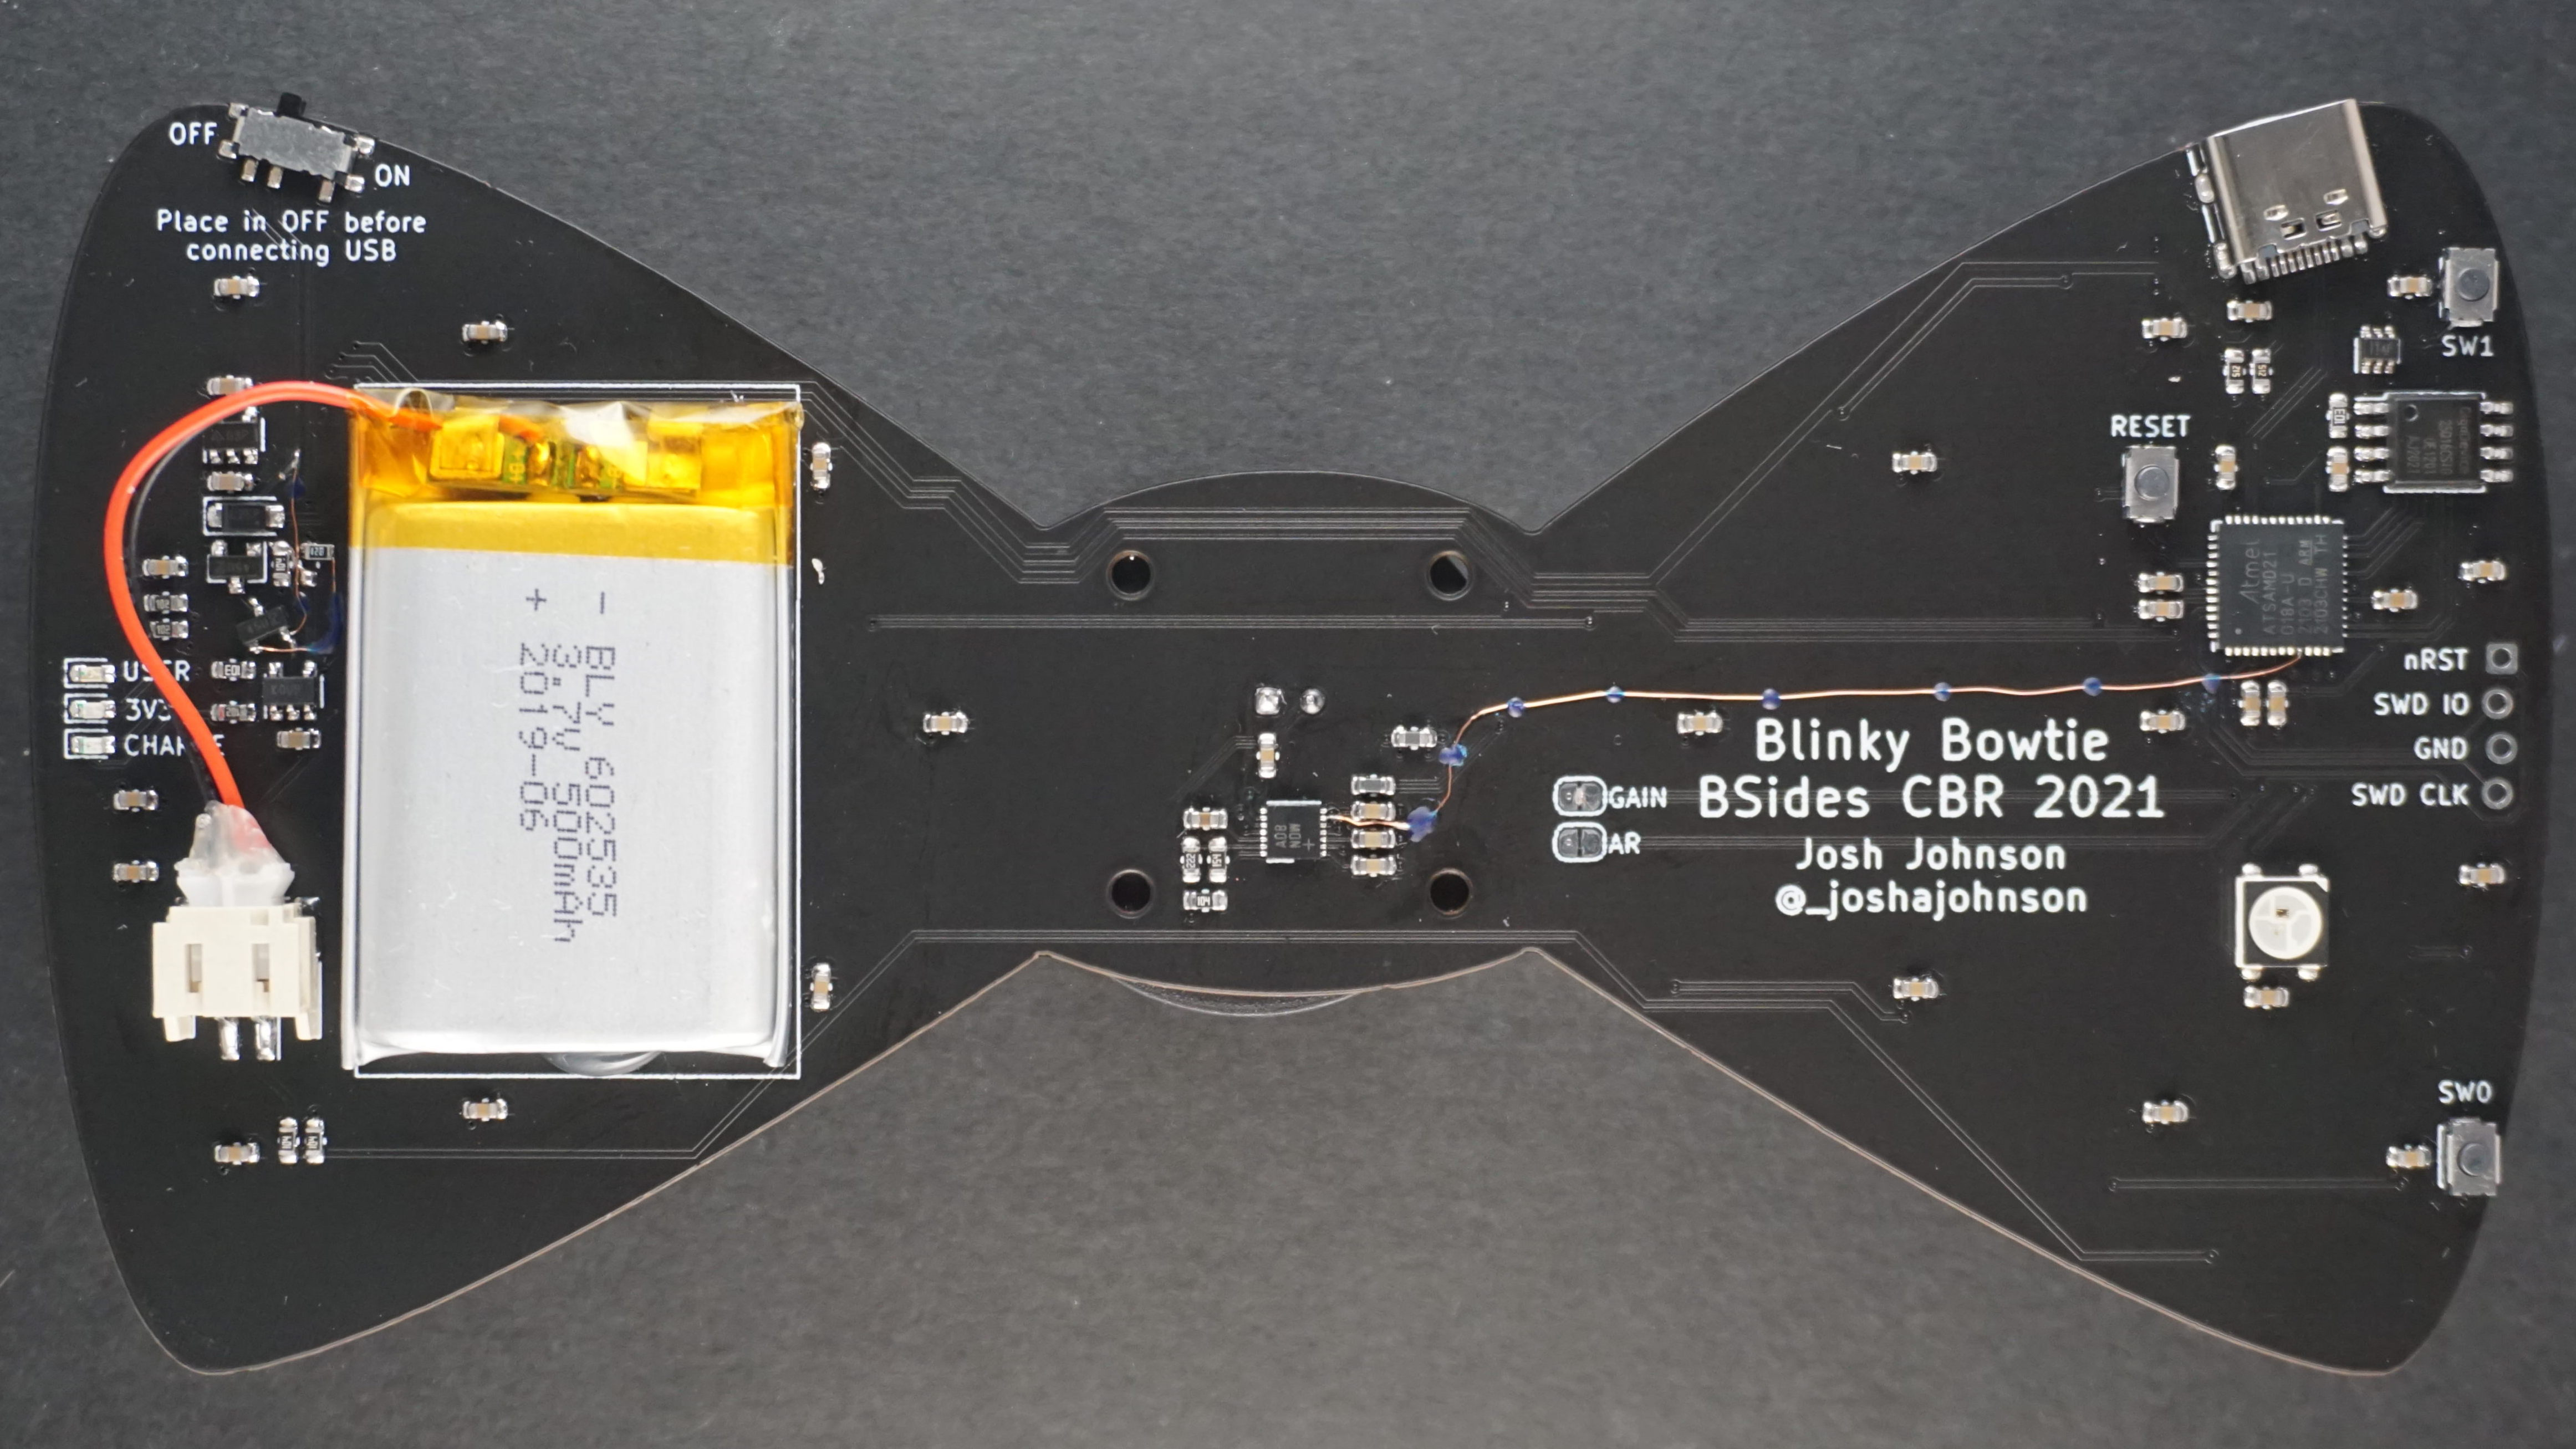
\includegraphics[width=0.8\linewidth]{images/bowtie-back.JPG}
	\end{figure}
\end{columns}
\end{frame}

%----------------------------------------------------------------------------------------
\begin{frame}
\frametitle{Integrated Design - Schematic}
\vspace{-5mm}
\begin{columns}
	\column{.4\textwidth}
	\begin{itemize}
		\item Replicating Feather M0 and microphone breakout in addition to connections.
		\item Numerous symbols had to be designed from scratch.
		\item Numerous new features including power control, buttons.
		\item Risk of transcription errors from module schematics and higher chance of miswiring components.
		\item 30 unique parts, 92 parts total.
	\end{itemize}
	\column{0.59\textwidth}
	\begin{figure}
		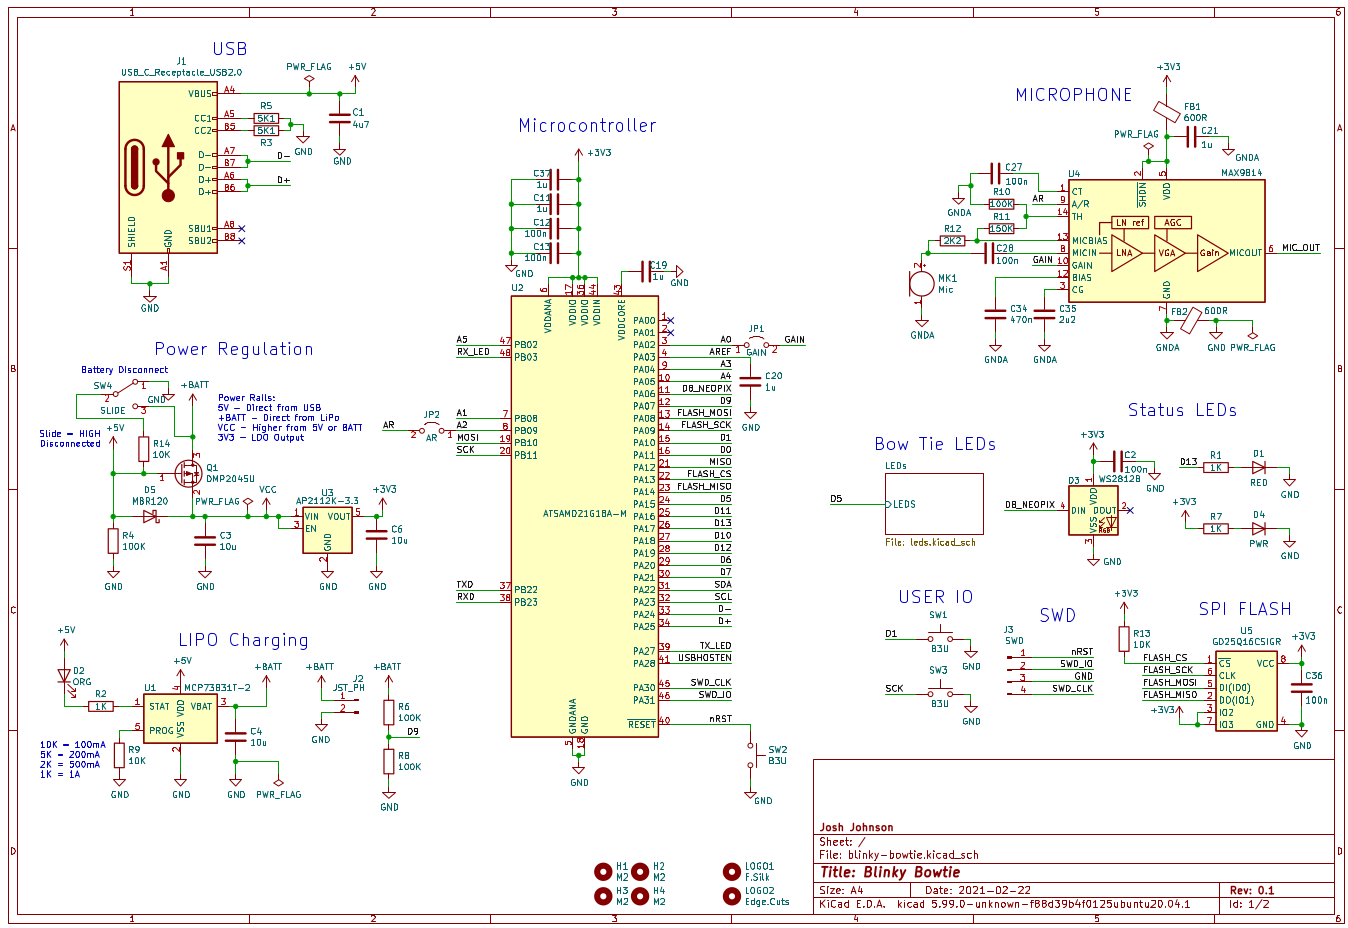
\includegraphics[width=\linewidth]{images/integrated-schematic.png}
	\end{figure}
\end{columns}
\end{frame}

%----------------------------------------------------------------------------------------
\begin{frame}
\frametitle{Integrated Design - Layout}
\vspace{-5mm}
\begin{columns}
	\column{.5\textwidth}
	\begin{itemize}
		\item Two layer board, signals and power pour on bottom, ground pour on top.
		\item Primarily 0603 passives and leadless IC's.
		\item Double sided assembly - LEDs and microphone on front, remainder on back.
		\item Complex board outline and artwork imported from Inkscape.
		\item Fully 3D modeled, allowing design of the mounting mechanism and identification of part interference.
	\end{itemize}
	\column{0.49\textwidth}
	\begin{figure}
		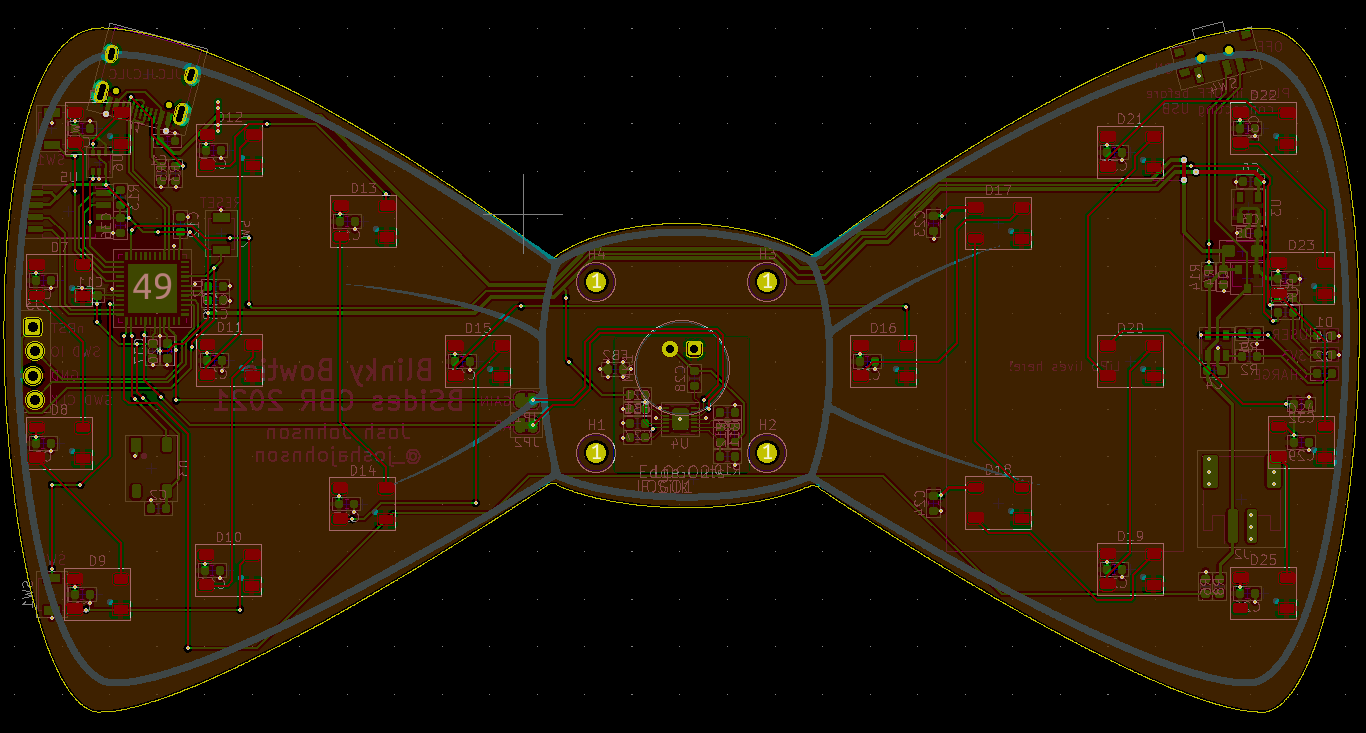
\includegraphics[width=0.9\linewidth]{images/bowtie-layout.png}
		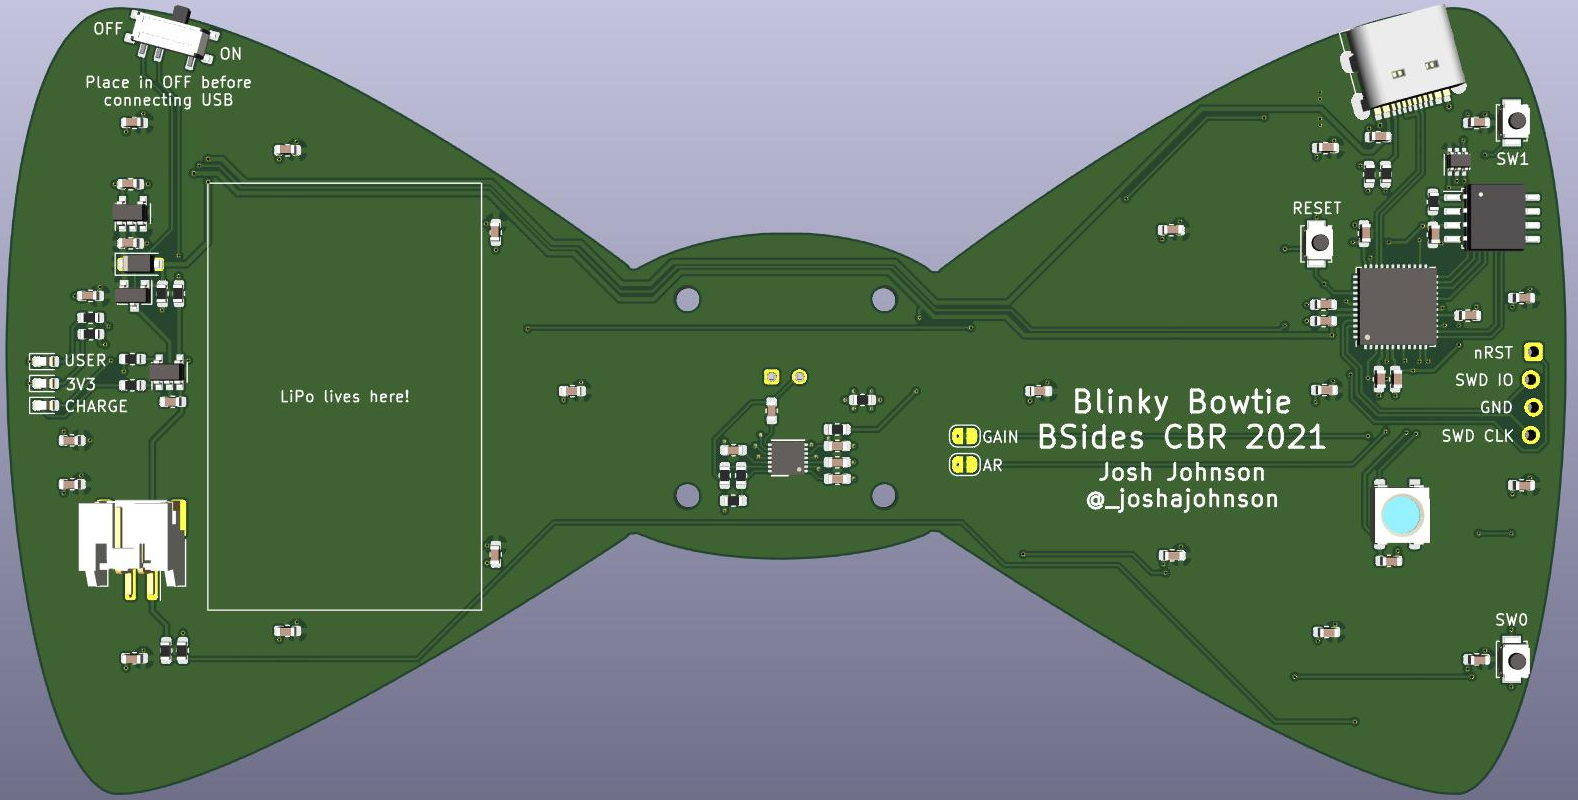
\includegraphics[width=0.9\linewidth]{images/bowtie-render.jpg}
	\end{figure}
\end{columns}
\end{frame}

%----------------------------------------------------------------------------------------
\begin{frame}
\frametitle{Integrated Design - Assembly}
\vspace{-5mm}
\begin{columns}
	\column{.5\textwidth}
	\begin{itemize}
		\item Double sided reflow assembly using a solder paste stencil.
		\item Required reflow oven, stencil, solder paste, hot air, microscope, and soldering iron.
		\item Used the "Interactive HTML BOM" tool to help identify part locations.
		\item Bootloader flashed using external programmer, then firmware via USB.
		\item Numerous hardware issues requiring flying wires, along with bootloader issues made initial bringup take three days.
		\item Feature additions and fine tuning took another day.
	\end{itemize}
	\column{0.49\textwidth}
	\begin{figure}
		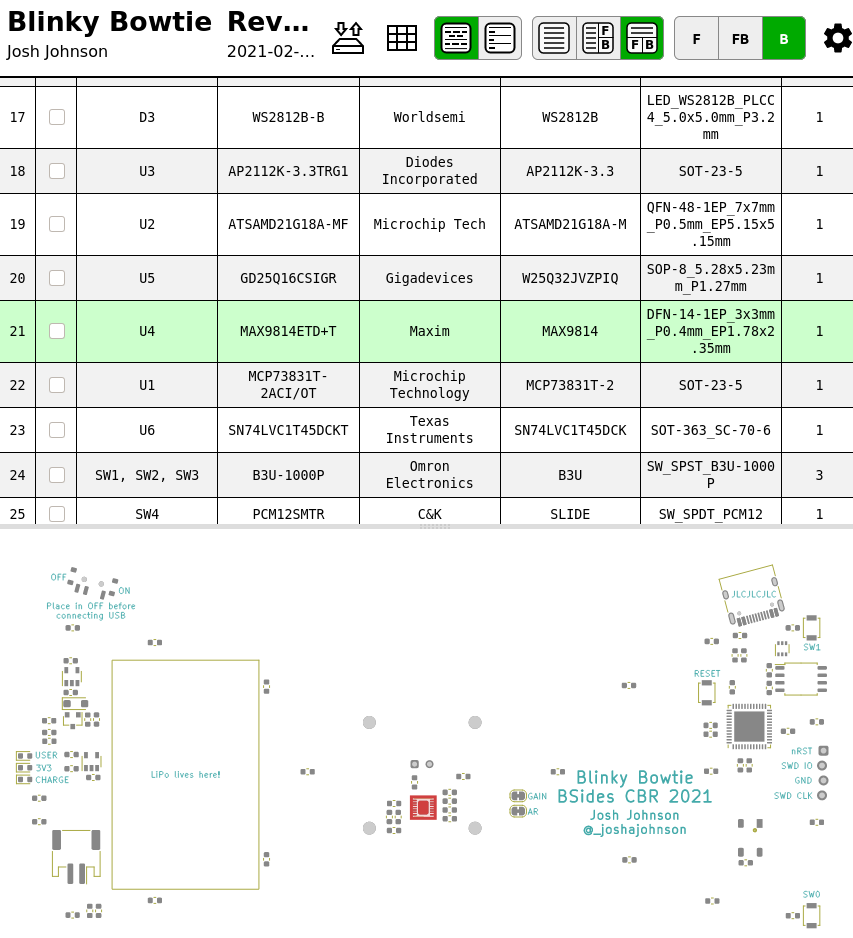
\includegraphics[width=\linewidth]{images/ibom.png}
	\end{figure}
\end{columns}
\end{frame}

%----------------------------------------------------------------------------------------
\begin{frame}
\frametitle{Flying Wire: Microphone Amp to MCU}
	\begin{figure}
		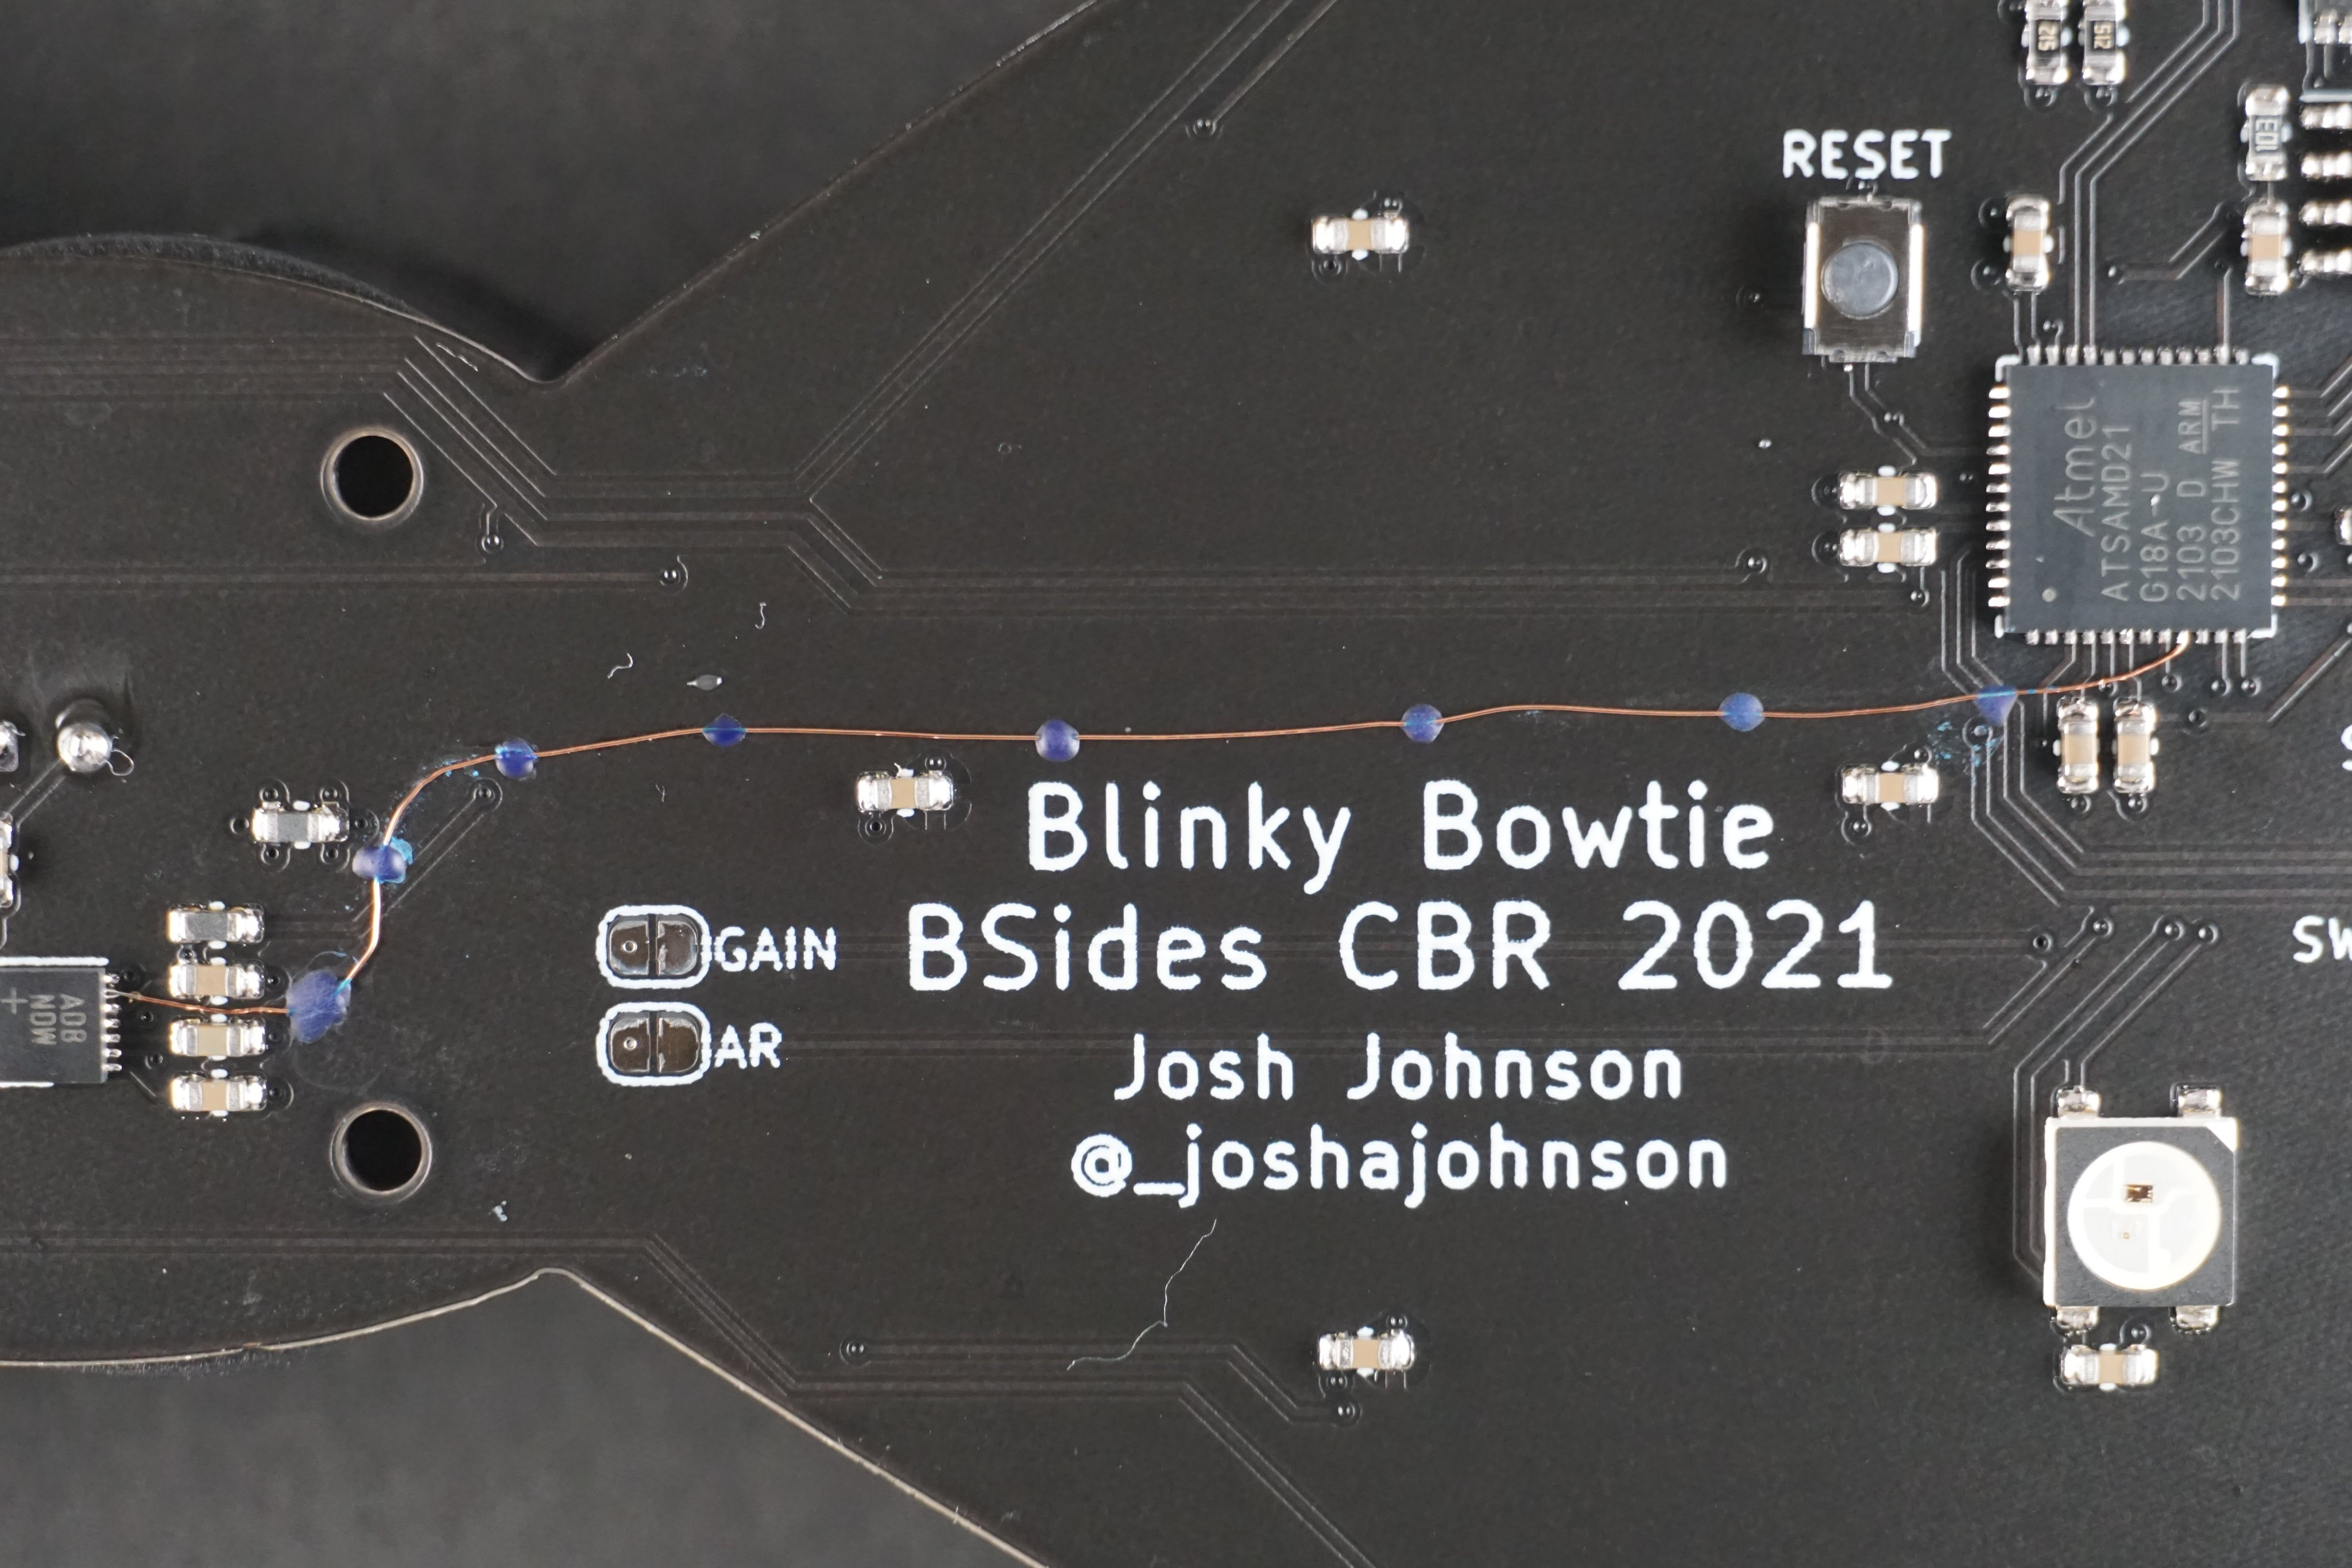
\includegraphics[width=0.7\linewidth]{images/bowtie-long-wire.jpeg}
	\end{figure}
\end{frame}

%----------------------------------------------------------------------------------------
\begin{frame}
\frametitle{Bodge: Power Selection}
	\begin{figure}
		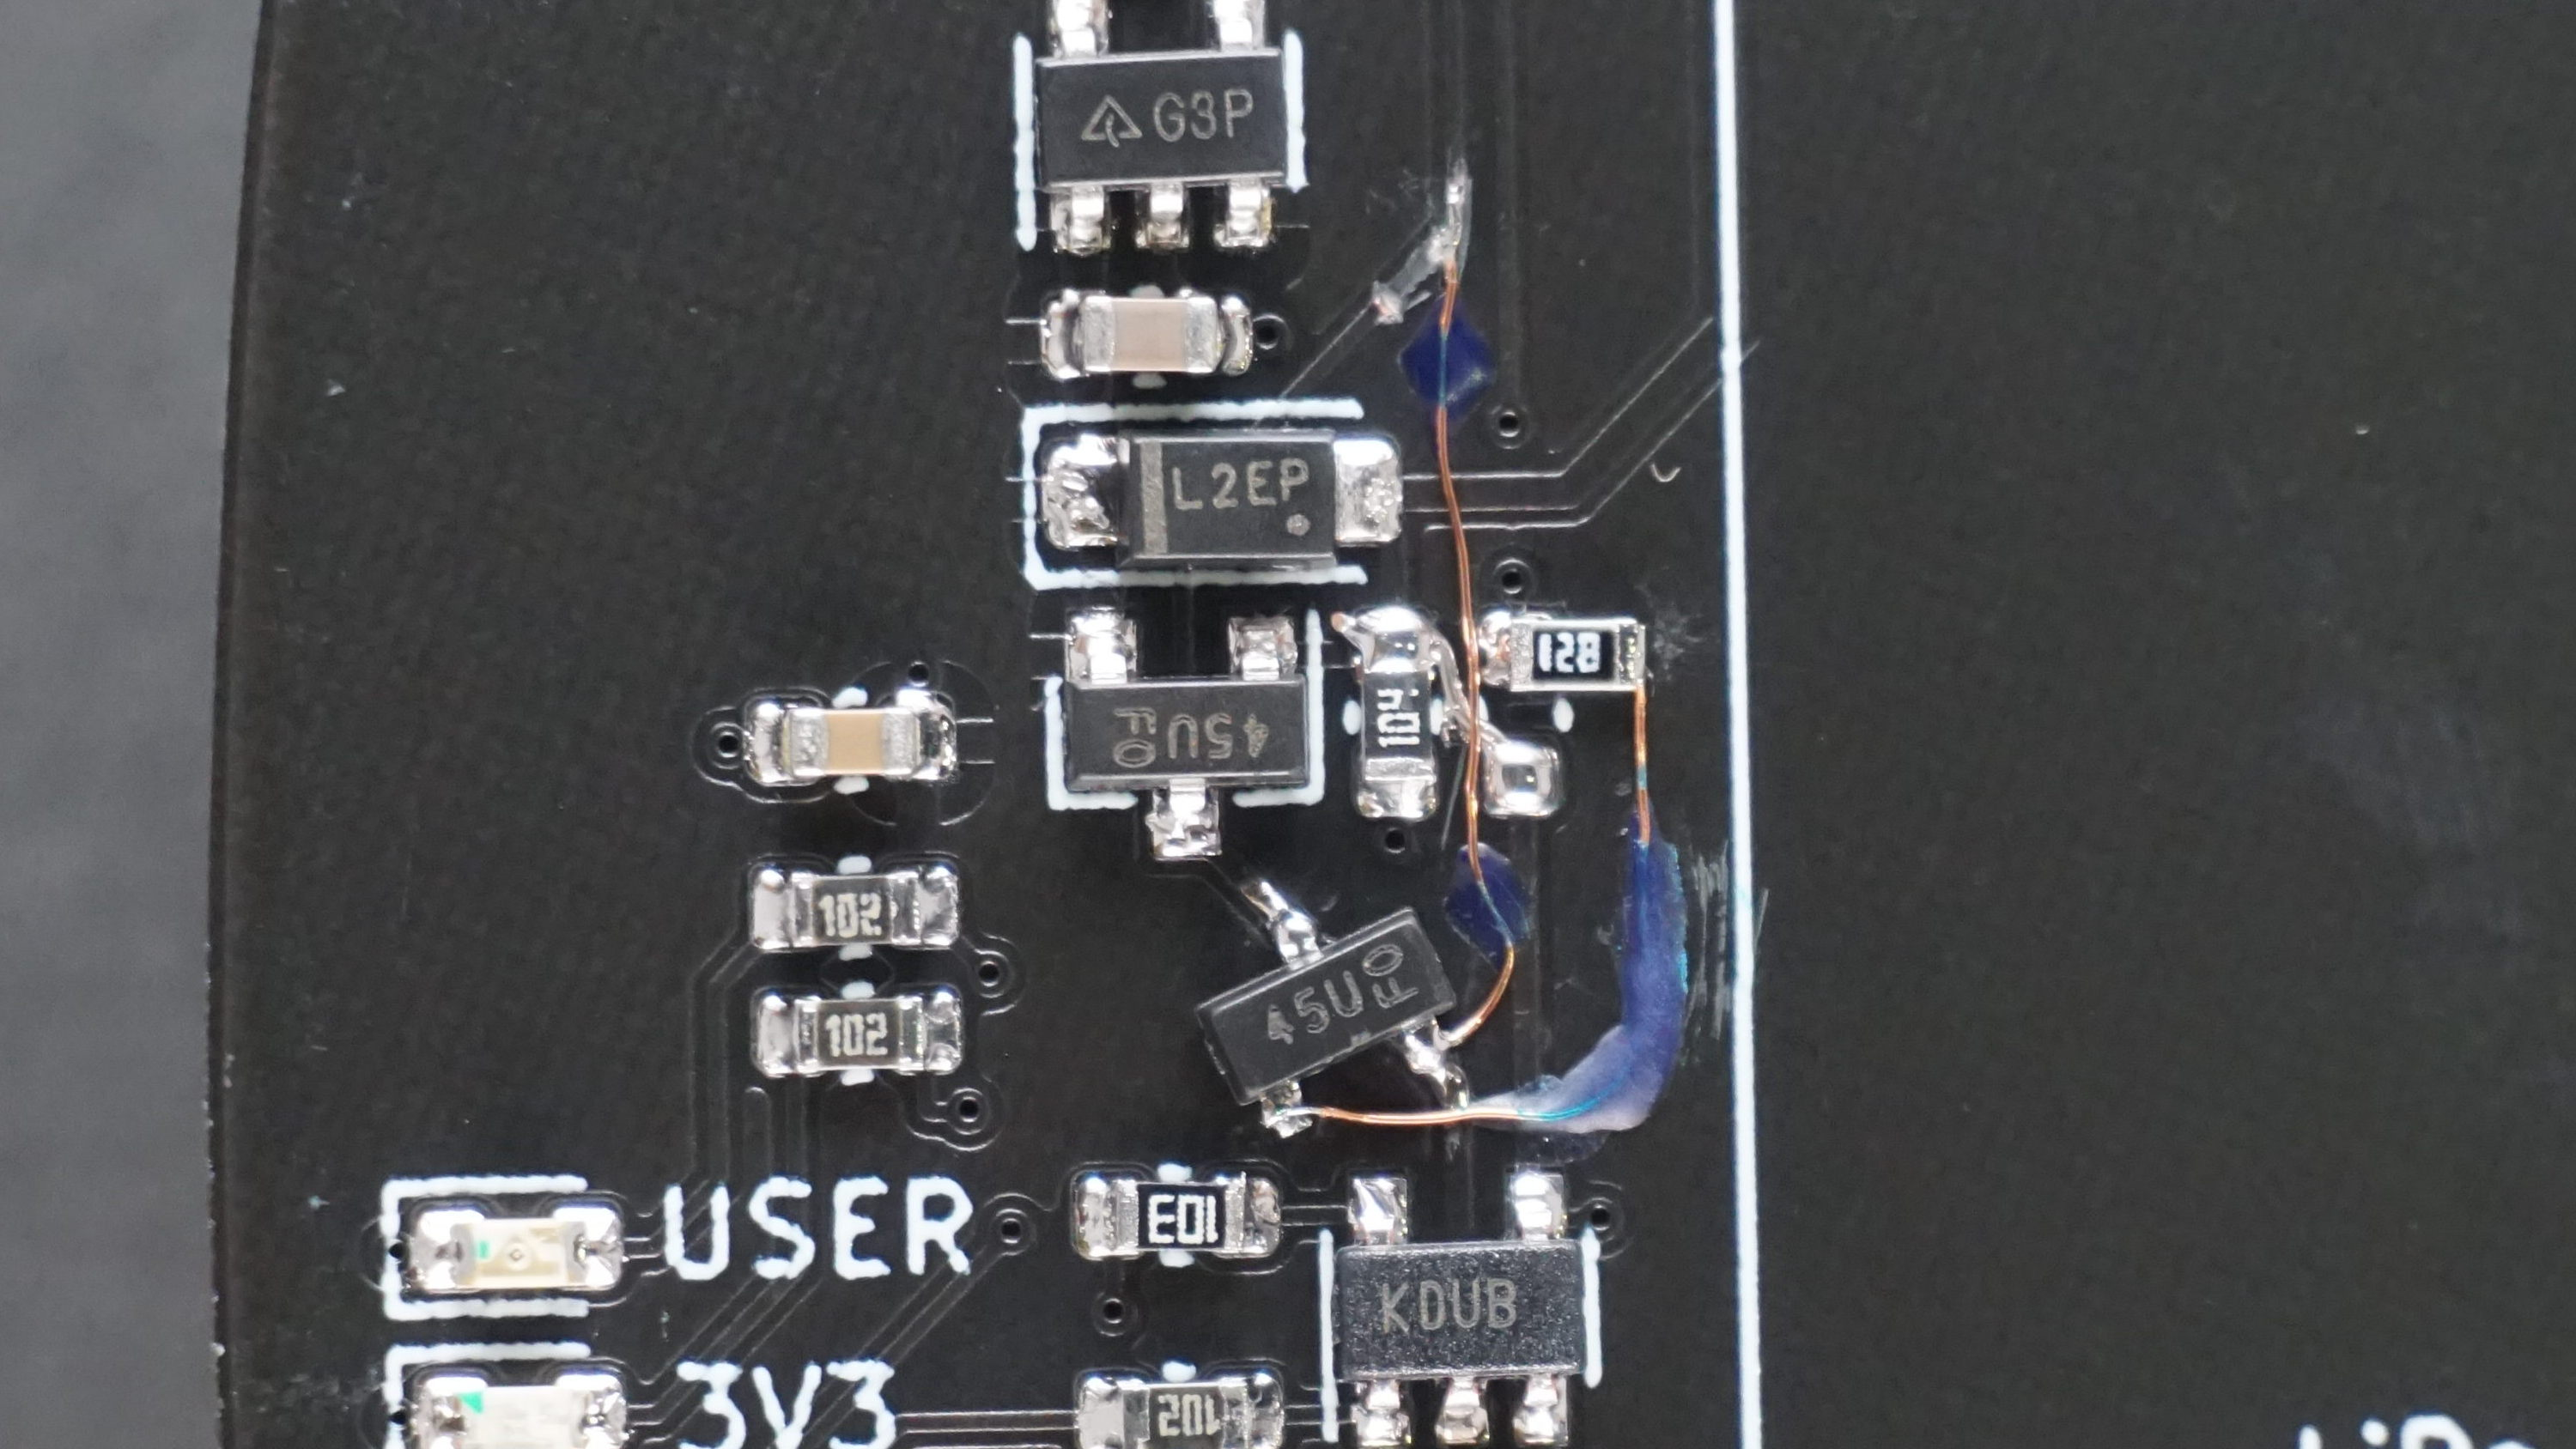
\includegraphics[width=0.8\linewidth]{images/bowtie-power.JPG}
	\end{figure}
\end{frame}

%----------------------------------------------------------------------------------------
\begin{frame}
\frametitle{Other Projects}
\vspace{-5mm}
\begin{columns}
	\column{.5\textwidth}
	\begin{figure}
		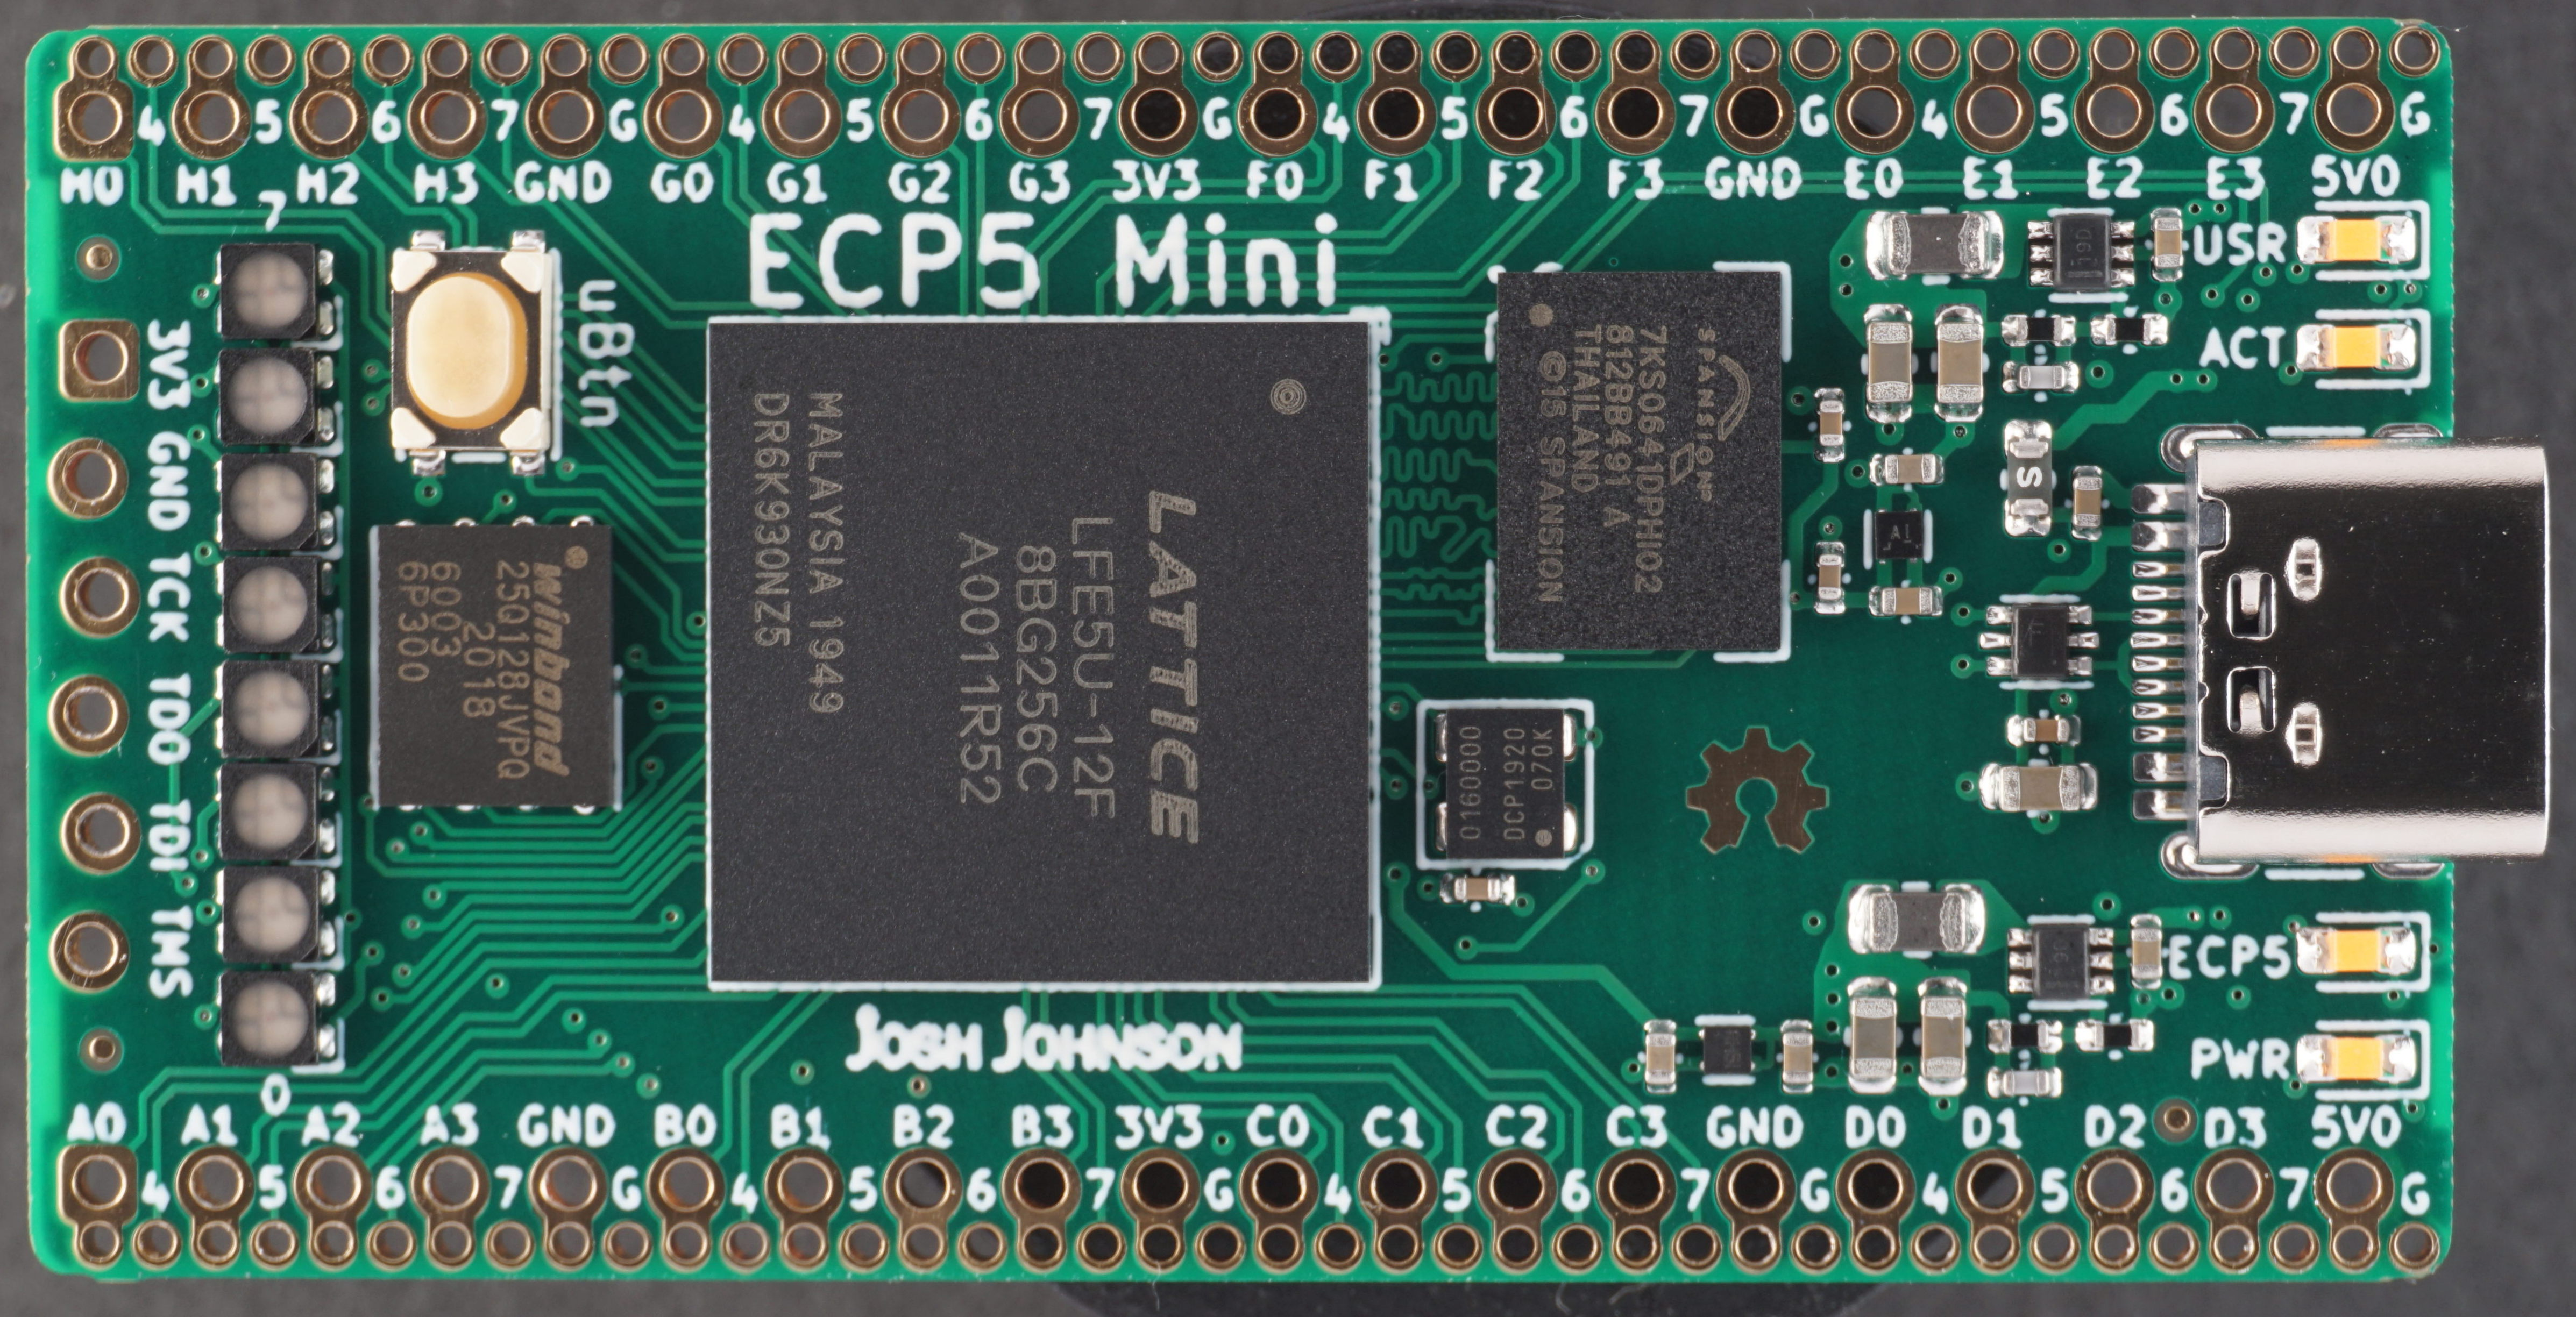
\includegraphics[width=0.95\linewidth]{images/ecp5-front.JPG}
		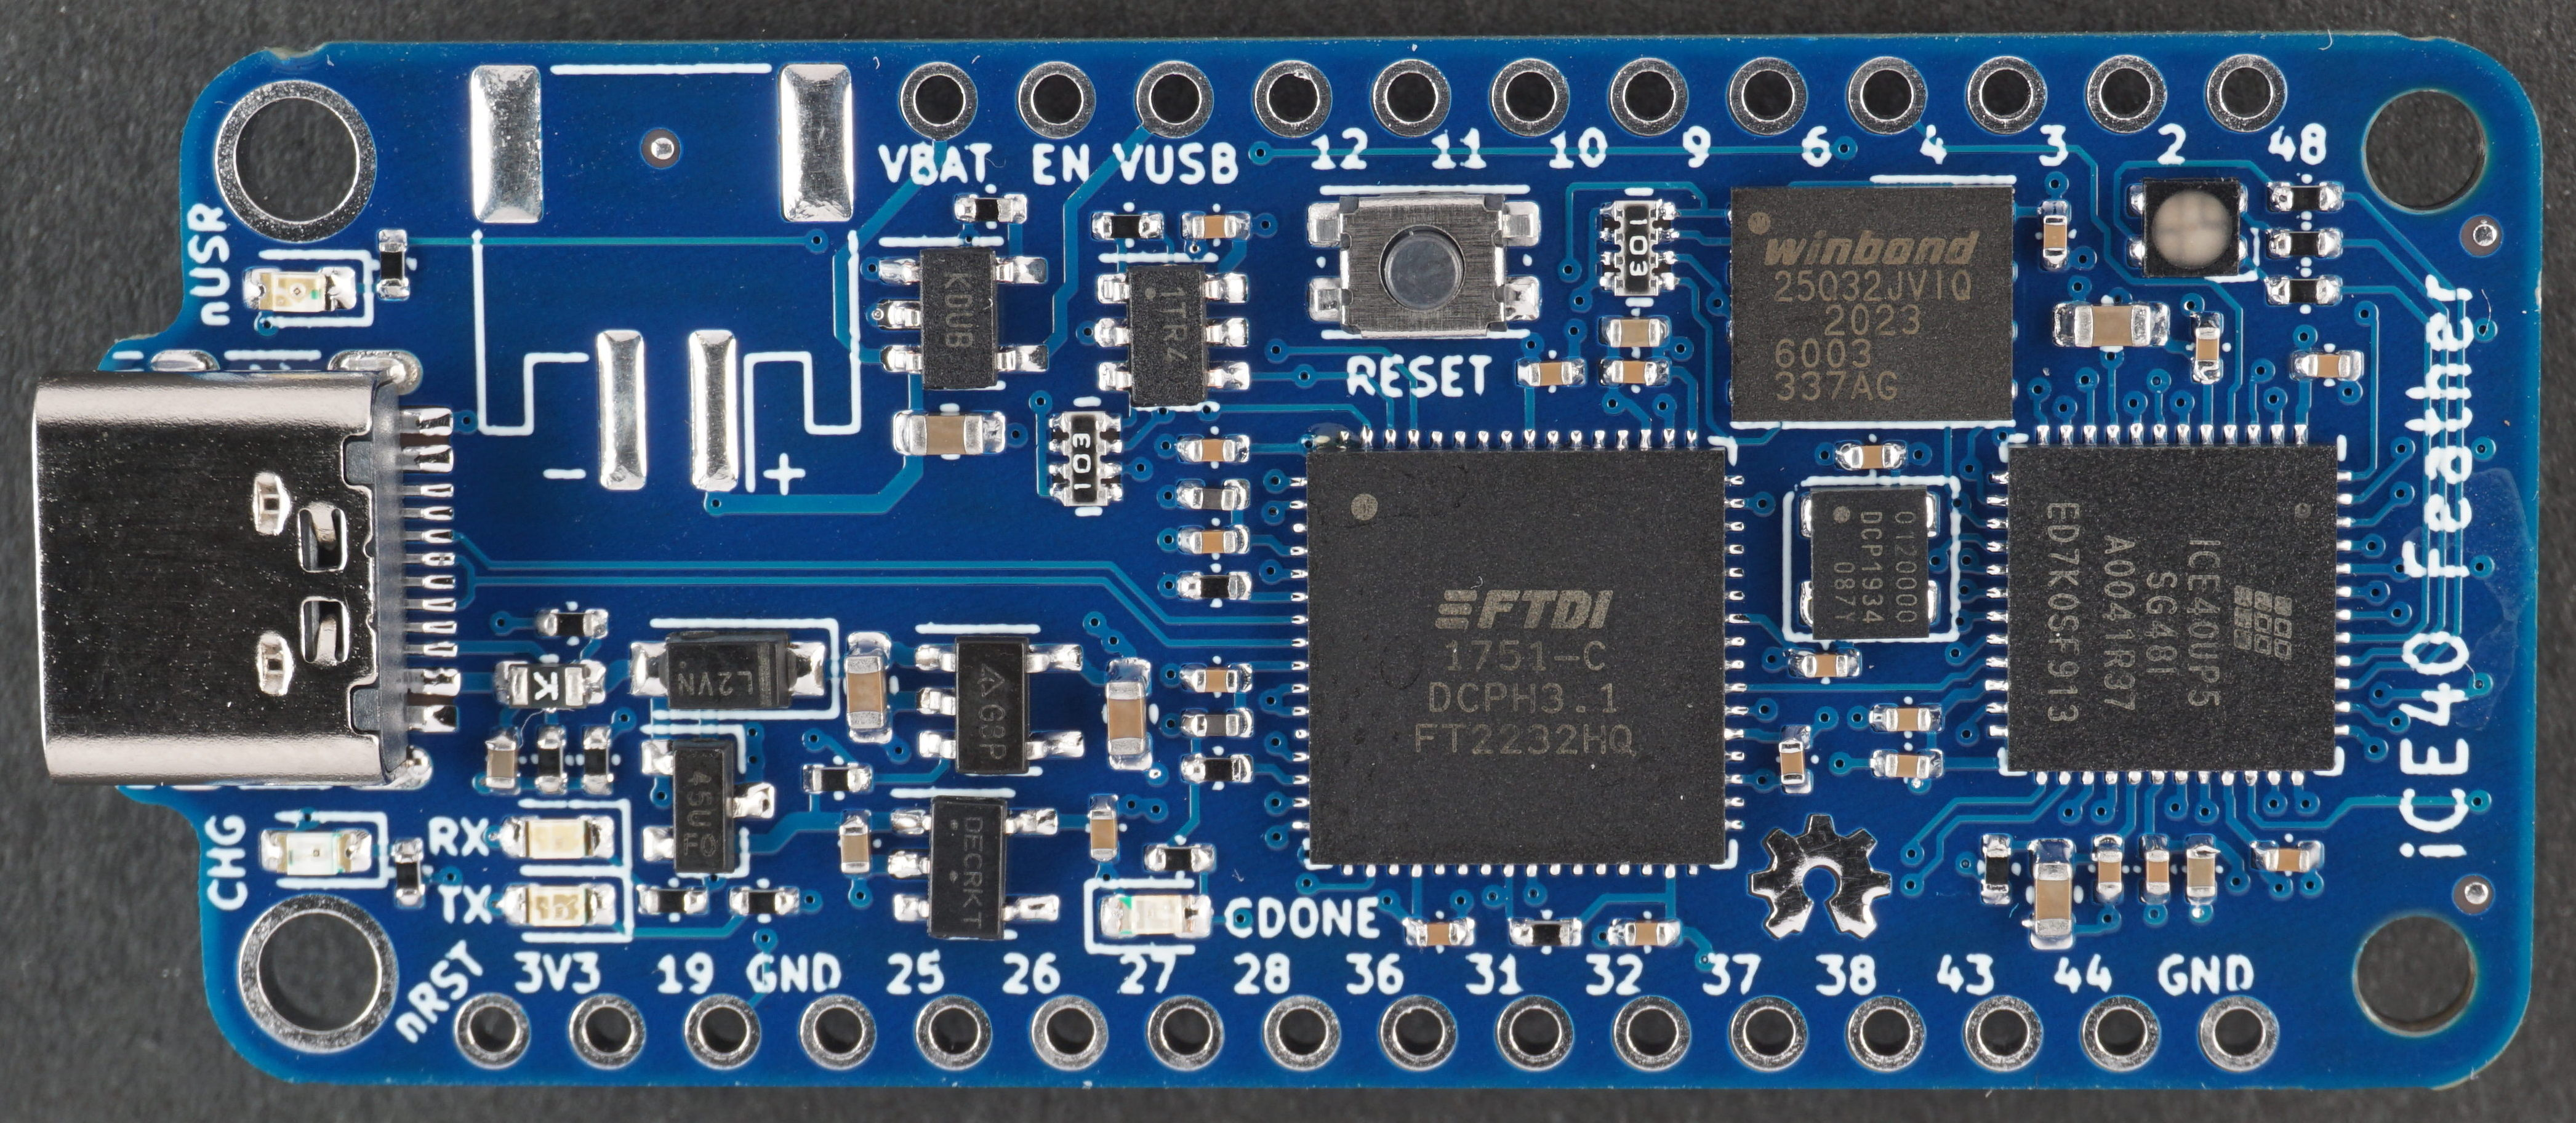
\includegraphics[width=0.95\linewidth]{images/ice40.JPG}
	\end{figure}

	\column{0.49\textwidth}
	\begin{figure}
		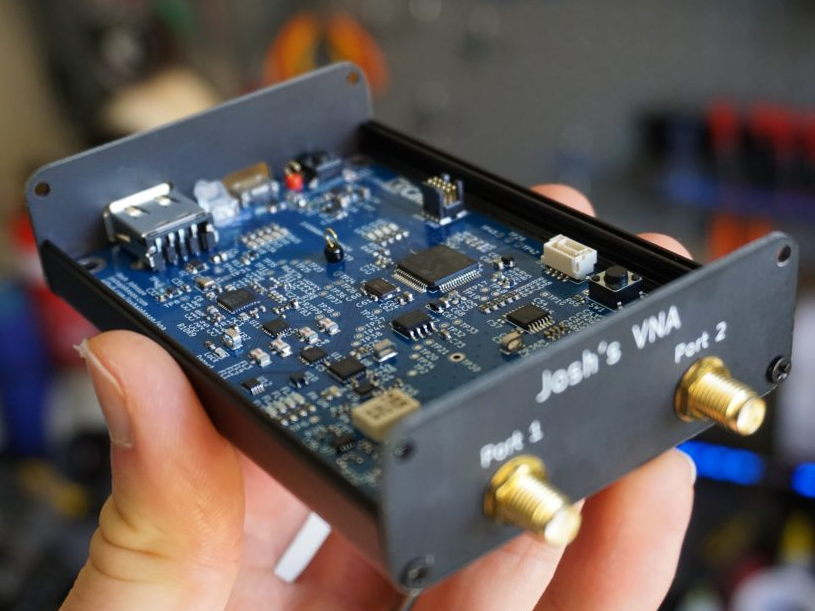
\includegraphics[width=0.825\linewidth]{images/vna.jpg}
		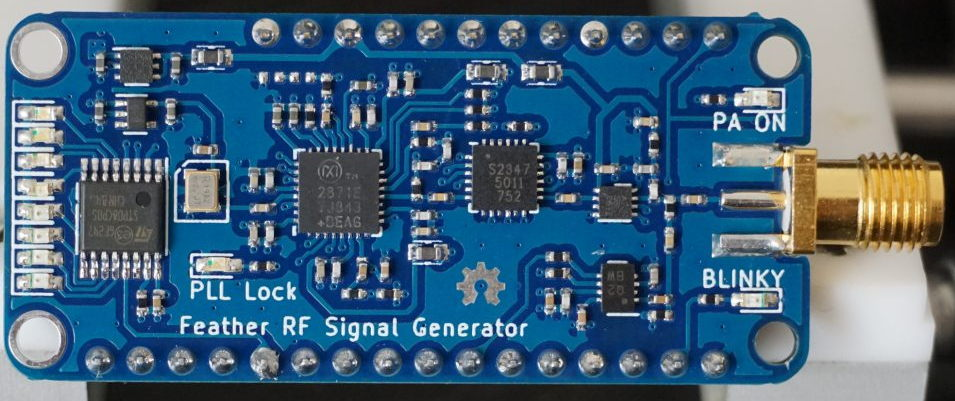
\includegraphics[width=0.825\linewidth]{images/rf-sig-gen.jpg}
	\end{figure}
\end{columns}
\end{frame}

%----------------------------------------------------------------------------------------
\begin{frame}
\frametitle{Questions?}
Slides and supporting documentation: \url{github.com/joshajohnson/bsidescbr2021}\\[10pt]
Repo contains all KiCad source files, images, and links if you want to learn more.\\[10pt]

\begin{columns}
	\column{.4\textwidth}
	\ Please say hello!\\[10pt]
	\ Twitter: @\textunderscore joshajohnson\\
	\ BSidesCBR Slack: josh\\
	\ Email: josh@joshajohnson.com\\

	\column{0.59\textwidth}
	\vspace{-8mm}
	\begin{figure}
		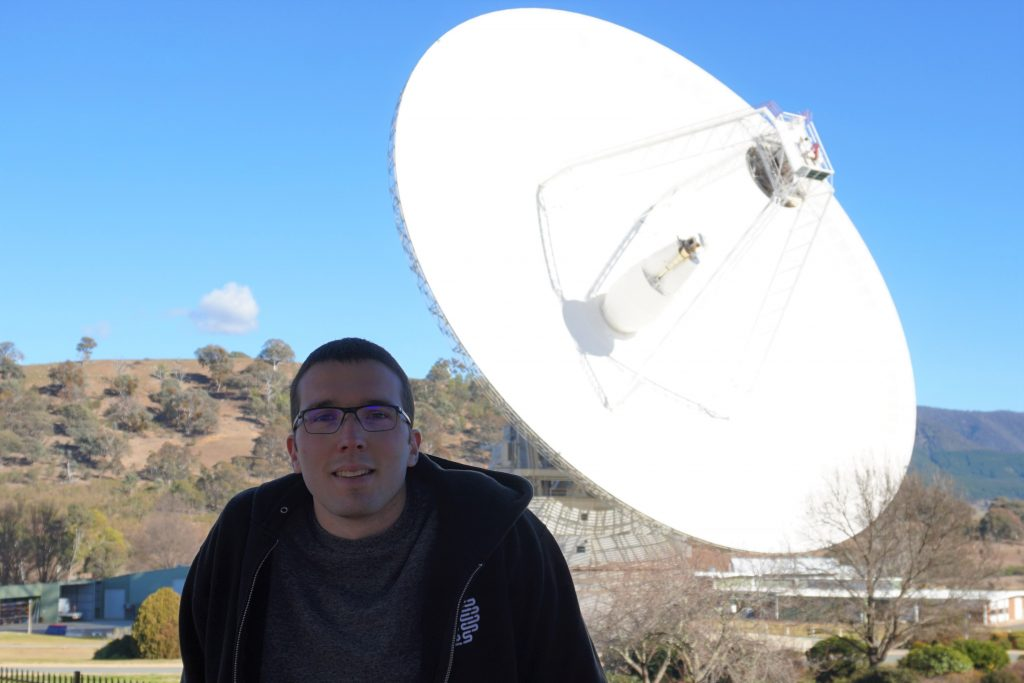
\includegraphics[width=0.925\linewidth]{images/josh-mugshot.jpg}
	\end{figure}
\end{columns}
\end{frame}
\end{document} 